%************************************************
\chapter{Patterns of sitewise selection in mammalian genomes}
\label{ch_mammals1}
\acresetall
%************************************************

\section{Introduction}

This chapter describes the use of sitewise evolutionary estimates to
characterize the global distribution of selective constraint across 38
mammalian genomes and within the major mammalian superorders. I apply
the \ac{slr} test, which was introduced in Chapter \ref{ch_intro} and
evaluated in Chapter \ref{ch_indels1}, to the set of mammalian
orthologous gene trees from Chapter \ref{ch_orthologs} to generate
genome-wide sets of sitewise statistics measuring selective constraint
in several groups of \mammln species. Both this chapter and the
following one are concerned with the analysis of these \sw data: here
I will consider the overall distribution of constraint observed in
several groups of mammalian genomes, while Chapter \ref{ch_mammals2}
will look at the use of these \sw data to identify trends in the
evolution of genes and protein domains.

The first section of this chapter describes the preparation and
alignment of the mammalian orthologs from Chapter \ref{ch_orthologs}
and introduces a protocol for filtering genome-wide sitewise
estimates. Although the simulations from Chapter \ref{ch_indels1}
showed that sequences with divergence levels above that of most
mammalian proteins can be aligned without introducing many false
positives due to misaligning biological insertions and deletions, the
analysis of empirical sequence data involves many potential
non-evolutionary sources of alignment error. A sequenced and annotated
genome is not a piece of observed data; rather, it is the result of a
succession of inferences (based ultimately on the observation of a
pool of genomic DNA by some sequencing technology), each step along
the way involving potential errors and biases. Chapter
\ref{ch_orthologs} looked at the identification of mammalian
orthologs, showing that the inference of correct gene trees can be
fraught with difficulties, and that \lcv genomes are under-represented
in gene duplications. Other sources of error, including those
occurring while sequencing DNA bases, assembling genomic fragments,
and annotating gene-coding regions have all been previously
highlighted as being important in the large-scale analysis of genomic
data \citep{TODO}. As such, care was taken to design and evaluate a
variety of filters to reduce the probability of yielding misleading
results.

The second portion of this chapter looks at the global distribution of
mammalian selective constraint, using \sw estimates to identify sites
evolving under purifying and positive selection at various confidence
levels. In parallel with the major goal of the \ac{mgp} to understand
the amount of evolutionary constraint across the entire mammalian
genome, the purpose of this analysis was to better understand the
distribution of evolutionary constraint within mammalian
protein-coding regions, focusing on what proportion of protein-coding
material has been evolving under purifying, neutral, or positive
selection in mammals. Proteins are well understood to evolve under
strong purifying constraint due to their functional importance
\citep{Fay2003}, but some regions of proteins, such as disordered
regions between two well-folded domains, may evolve under relaxed
constraints. Furthermore, positive selection of beneficial
substitutions can also play a role in shaping the evolutionary history
of proteins \citep{Pal2006}. There has thus been great interest in
understanding the role of adaptive evolution in shaping the genes and
genomes of mammals and primates, but different studies have produced
widely varying estimates of the number of genes subject to positive
selection \citep{MarquesBonet2009a,Ellegren2008}.

While most previous investigations of positive selection in mammals
have focused on the gene as the unit of analysis, the current analysis
used a primarily \sw approach. The focus on identifying \acp{psc}
instead of the traditional identification of \acp{psg}, allowed for a
more flexible quantification of levels of purifying and positive
selection in mammals. One expected benefit of the \sw approach was
that fine-grained filtering on a site-by-site basis could be performed
both before and after the computationally expensive step of estimating
evolutionary parameters, allowing for a more extensive and flexible
set of filters to be used in estimating the potential impact of
alignment or annotation error on the amounts of inferred positive
selection.

%The second, more subtle goal of this analysis was to place the
%distribution of selective pressures implied by the \sw analysis within
%the context of previous population genetic and comparative
%studies. Many population genetic studies have analyzed the
%distribution of selective pressures resulting from mutations in
%protein-coding regions, known as the \ac{dfe}. Analyses of variation
%data from \emph{Drosophila} have found that relatively few amino acid
%substitutions in \emph{Drosophila} are effectively neutral, while up
%to 50\% have apparently been due to positive selection
%\citep{Loewe2006,EyreWalker2007}; similar studies based on variations
%in humans have indicated a much lower fraction of positively-selected
%substitutions in our recent evolutionary history
%\citep{EyreWalker2006a,Boyko2008}. This is in line with the
%expectation, based on population genetic theory, that species with
%higher effective population sizes experience more effective natural
%selection \citep{EyreWalker2007}. As \emph{Drosophila} has
%historically had a much larger effective population size than humans
%and most mammals (e.g., on the order of 10$^{6}$ for \emph{Drosophila}
%vs. 10$^{3}$ for humans), one would expect to see more neutral
%evolution, and less purifying and positive selection, in human
%protein-coding regions.

%Although there is a strong theoretical connection between the \ac{dfe}
%commonly from population genetics and the \dnds ratios more commonly
%estimated in comparative analyses, only one study, performed by
%Nielsen and Yang \citeyearpar{Nielsen2003}, has explicitly estimated
%the \ac{dfe} using data from fixed differences between species. Using
%data from primate mitochondrial genomes, Nielsen and Yang found that a
%variety of two-parameter distributions for the \ac{dfe} fit the
%dataset equally well and that none of the best-fit distributions
%contained a large amount of probability mass within the range of
%purely neutral or beneficial selection coefficients; most of the
%distribution was contained within the range of moderately deleterious
%selection coefficients (e.g., $-3<S<-1$, corresponding roughly to
%\dnds values between 0.2 and 0.6). Unfortunately, no attempt has since
%been made to use comparative data to estimate the \ac{dfe}; as a
%result, one goal of this analysis was to determine whether \sw
%estimates could successfully be used to infer the \ac{dfe}. Though the
%methods I employed for this analysis differed strongly from the
%approach of Nielsen and Yang, a comparison to their results could
%validate the use of \ac{slr} for estimating the \ac{dfe}. Furthermore,
%it would be interesting to understand whether the differences in
%historical effective population sizes between mammalian subgroups,
%which have been shown repeatedly to affect overall \dnds levels in
%primates versus rodents \citep{Kosiol2008,Ellegren2009}, has a
%detectable impact on the \ac{dfe} inferred from comparative
%data. Although the effective population size differences between
%mammalian subgroups are far smaller than the difference between
%mammals and species like \emph{Drosophila}, a comparison of the
%\ac{dfe} from different mammalian groups could be used to evaluate how
%strong of an impact the effective population size has on the
%proportion of protein-coding sites subject to varying levels of
%natural selection.

\section{Data quality concerns: sequencing, assembly and annotation error}

\subsection{The impact of sequencing errors on error rates in detecting positive selection}
\label{sec_error_impact}

The possibility that erroneously-aligned sequences might cause false
positives in the detection of sitewise positive selection was a major
concern for this analysis, especially given the \lcv nature of the 20
newly-sequenced genomes. Although the \slr test and other \sw \ml
methods have been shown to be conservative in their identification of
positively selected sites under most conditions, even when the amount
of data is low or the null model is violated
\citep{Anisimova2002,Anisimova2003,Massingham2005}, most evolutionary
analyses are based on the assumption that all sites within an
alignment column are truly homologous. This assumption can be violated
in a number of ways.

Of course, alignment error can result from errors in reconstructing
the evolutionary history of sequences evolving with indels, causing
non-homologous codons to be placed in the same alignment column. In
Chapter \ref{ch_indels1} I explored the tendency of a number of
progressive multiple alignment programs to produce such errors,
showing that \prankc alignments introduce few falsely identified
positively-selected sites resulting from alignment errors at
mammalian-like divergence levels. Thus, \prankc was used to align all
coding sequences, and the number of false positives resulting from
misalignment of biological insertions and deletions was expected to be
low.

Biological indels are not the only potential source of misalignment
error. Errors resulting from the inclusion of incorrect genomic
sequence in coding sequences were an additional concern. The \lcv
genomes were not assembled into chromosomes and had large amounts of
missing sequence, making the likelihood of miscalled bases, spurious
insertions or deletions, or shuffled regions due to mis-assembly
relatively high \citep{Green2007}. The magnitude of the effect of each
of the aforementioned types of sequence errors on the detection of
positive or purifying selection depends on the nature of the inference
method, the type of sequencing error, and the branch length of the
terminal lineage leading to the species containing the sequence error.

As most codon-based inference methods assume independence between
amino acid sites, the effect of misalignment on the resulting
inference will be independent between neighboring codons. Thus, one
may first consider the effect---in isolation---of a single
spuriously-assigned homologous codon on the \ml estimation of
\omg. Two distinct situations can be encountered: first, the case
where a single sequence error causes one spurious nucleotide
substitution within a codon, and second, the case where one or
multiple sequence or assembly errors cause multiple spurious
substitutions within a codon. Single spurious nucleotides, such as
miscalled bases, would add noise to the estimation of \omg, but as a
whole they would not be expected to cause false positive \acp{psc}. If
we assume no large difference between the natural mutational process
and the process that caused the erroneous mutation (e.g., a random
distribution across codon positions and no bias in the identity of the
miscalled base) then the effect would be to shift the estimated \omg
in the branch containing the error towards 1. This is because, on
average, isolated miscalled bases would appear the same as a neutral
substitution process, inflating the estimated substitution rate but
not affecting the relative \nsyn and \syn rates.

In contrast to single spurious substitions, codons with multiple
erroneous bases in one species may produce strongly elevated inferred
substitution rates and \omg estimates. This is due to the necessity of
the codon model implemented in SLR to infer a multi-step path of
single substitutions between the two codons on either side of a given
evolutionary branch. The exact \ml path estimated between two
completely non-homologous codons depends on the estimated codon
frequencies, the branch length separating the two sequences, and the
nature of the process causing misalignment of nonhomologous codons,
but in general it would be reasonable to expect a greater number of
false positive \acp{psc} resulting from codons with multiple erroneous
bases than from codons with single errors due to the necessary
inference of a multi-step path between codons with multiple nucleotide
differences.

Given the potentially greater impact of codons with multiple errors,
the propensity of each of the common sequencing error types identified
above (miscalled bases, spurious indels, and
shuffled/repeated/collapsed regions due to mis-assembly) to cause
single or multiple errors within codons could strongly affect its
impact on the sitewise detection of positive selection. On its own, a
miscalled nucleotide base would obviously result in a single spurious
substitution. However, low-quality bases tend not to be uniformly
distributed among or within sequence reads \citep{Kircher2009},
leading to an increased probability of multiple errors within a codon
resulting from miscalled bases. Spurious indels within coding regions
may be even more likely than miscalled bases to cause multiple errors
within a codon due to the potential for creating frameshift
artifacts. Assembly errors, which result in larger-scale structural
errors including missing, repeated, shuffled or inverted sequence
regions \citep{Jaffe2003}, are especially prone to producing codons
with multiple erroneous substitutions due to the large amount of
contiguous sequence data being misplaced.

For detecting positive selection, the specific test used and the
branch lengths separating the species being tested may also have an
impact on the prevalence false positives resulting from sequence
errors. Sequence errors should only substantially affect the
estimation of \nsyn and \syn substitution rates along the terminal
lineage leading to the erroneous sequence data; thus, the potential
impact of sequencing error on the inference of a positively selected
site or gene can be estimated by considering the potential impact of
an inflated rate of \nsyn substitution along the terminal branch on
the inference of positive selection with a given test. Both the
branch-site test for positive selection (which was not used in this
analysis) and the sitewise tests for positive selection (including
\pamlEight and \slr) are
sensitive to erroneous substitutions occurring at individual alignment
columns, with the major difference between the two types of test being
that the branch-site test is highly sensitive to substitutions along
the foreground branch(es) being tested for positive selection, while
sitewise tests only measure the signal for positive selection across
the entire evolutionary tree.

For the branch-site test, the potential effect of sequencing error
should depend on the location and length of the foreground branch(es):
if the terminal branch leading to the spurious sequence is within the
foreground, and especially if it represents a sizeable portion of the
overall foreground branch length, then false positives could easily
result; if, however, the terminal branch is outside of the foreground,
then it would have little direct impact on the \fpr of the branch-site
test aside from adding noise to the estimation of parameters in the
non-foreground branches of the tree.

For site-based tests such as \slr, the effect of sequencing error
should be independent of the position of the terminal branch within
the tree, depending more on the magnitude of \nsyn substitution rate
elevation resulting from the sequence error and the fraction of total
branch length covered by the ``erroneous'' terminal branch within the
phylogenetic tree being studied. It would be difficult to consider
each of these factors (the terminal branch length and the magnitude of
\nsyn substitution rate elevation) in isolation due to their
non-independence: sequence errors in a short terminal branch may yield
a strongly elevated \nsyn substitution rate, but the impact on the
overall inference of positive selection may be limited as a result of
the short branch length. On the other hand, the same erroneous
sequence in a species with a longer terminal branch would likely cause
a smaller elevation in the \nsyn substitution rate (due to the higher
expected number of substitutions along a longer branch) yet the impact
of such an elevated rate on the sitewise inference would be
proportionally greater due to the higher branch length. A reasonable
hypothesis would be that these opposing factors would effectively
cancel each other out in the \ml calculations. In either case, the
expectation that a phylogeny with a greater proportion of its branch
length within terminal branches (which, in contrast to internal
branches, may contain spurious substitutions resulting from sequencing
errors) would be more prone to false positives should still hold.
%To summarize, the expected effect of alignment errors on the sitewise
%detection of positive selection should be minimal when using a good
%aligner and analysing data within vertebrate divergence levels, but
%the number of false positives resulting from sequence errors depends
%on a number of factors including the frequency, spatial clustering,
%and terminal branch length associated with sequencing, assembly and
%annotation errors.
In some cases, even a relatively large amount of
sequencing error may not produce a strongly elevated \fpr (e.g., when
the total internal branch length is large as when analyzing all
mammals or vertebrates), as the addition of a few spurious
substitutions would not significantly change the estimated \nsyn
substitution rate. In other cases, however (e.g., when the branch
length is small or when many low-quality genomes are included), it may
significantly bias results towards excess false positives.

\subsection{Empirical evidence for a strong impact of sequencing, assembly and alignment error}

Simulation studies could improve our understanding of the relative
potential of different types of sequencing errors to introduce false
positives in downstream analyses, but the absolute frequency and
pattern of such errors would still difficult to predict without a
reliable model for their generation. This is especially true for
larger-scale errors from misassembly or misannotation, which are less
easily modeled than base calling errors and could have potentially
more significant negative effects. Instead, an empirical approach
seems more appropriate for quantifying the false positives resulting
from these types of sequence errors. In particular, two empirical
studies in mammals have provided convincing evidence that sequence,
alignment and annotation errors can drastically increase the number of
false positive \psg{}s in the branch-site test for positive selection.

Schneider et al. \citeyearpar{Schneider2009} performed a genome-wide
scan for positive selection in the terminal branches of 7 mammalian
genomes using the branch-site test and analysed the fraction of
\psg{}s within subsets of high- or low-quality genes according to
three sequence and alignment quality metrics. They found that the
fraction of \psg{}s was significnatly higher for genes exhibiting
lower quality sequence, annotation and alignment metric, with genes in
the highest-quality and lowest-quality categories showing a 7.2-fold
difference in the inferred fraction of \psg{}s
\citep{Schneider2009}. This observation provided evidence of a
correlation between the chosen quality metrics and the tendency of an
alignment to exhibit positive selection. It did not necessarily imply
causation, however, as the same result might have been observed---even
in the absence of sequence error---if some biological properties of
the true \psg{}s caused them to yield lower quality metrics than
non-\psg{}s. Looking at the three metrics used in their study
(sequencing coverage, gene annotation status, and alignment quality
according to the heads-or-tails method), it is plausible that
properties associated with elevated \omg ratios and positive
selection, such as recent gene duplication
\citep{Beisswanger2008,Studer2008,Casola2009}, high GC content
\citep{Ratnakumar2010} or functional shifts \citep{Storz2008,Wang2001}
might have had an error-independent effect resulting in a higher
proportion of \psg{}s in low-scoring categories. The heads-or-tails
method has also been shown to be inappropriate for estimating
alignment uncertainty \citep{Fletcher2010}, so results based on this
measurement should be taken with caution. Despite these criticisms,
the analysis did provide good evidence that some of the obvious
sources of error may be contributing to excessive estimates of
branch-specific positive selection in mammals.

\citet{Mallick2009} took a different approach to the same problem by
performing a careful resequencing and reassembly of the chimpanzee
genome (the initial assembly of which had lower coverage and lower
quality than the human genome) and re-analysing the evidence for
positive selection along the chimpanzee linegae in 59 genes which had
previously been identified as chimpanzee
\psg{}s. \citeauthor{Mallick2009}, who were motivated by a concern
that previous reports of a larger proportion of \psg{}s in chimpanzee
than in human \citep{Bakewell2007} were the result of its
lower-quality genome rather than a biologically significant difference
in levels of adaptation, found that the vast majority of \psg{}s
identified in two previous studies showed no evidence for positive
selection when using their reassembled and higher-coverage version of
the chimpanzee genome \citep{Mallick2009}. This suggested that the
original 4x coverage chimpanzee genome contained a number of
sequencing and assembly errors leading to false inferences of positive
selection. A detailed analysis of 302 codons with multiple spurious
\nsyn substitutions in the original assembly showed roughly comparable
effects of sequence error (explaining 23\% of codons), assembly error
(14\% of codons) and local alignment error (30\% of codons).

Taken together, the results of Schneider et
al. \citeyearpar{Schneider2009} and Mallick et
al. \citeyearpar{Mallick2009} provide strong evidence in support of
the hypothesis that errors in sequencing, assembly, annotation and
alignment can result in strongly elevated inferred \omg values when
using sensitive tests for detecting positive selection. Furthermore,
the detailed identification and quantification of error sources
performed by Mallick et al. \citeyearpar{Mallick2009} provided an
empirical estimate of how important each potential source of error
would be in the detection of positive selection. Although both of
these studies used the branch-site test for detecting positive
selection, their results could be expected to generalize well enough
to guide the design of filtering methods for the present \sw
analysis. With these results in mind, I implemented three filtering
steps to help identify and remove sequences and alignment regions
potentially subject to the errors noted above: filtering out
low-quality sequence, removing gene fragments and recent paralogs, and
identifying alignment regions with extremely high numbers of clustered
substitutions.

\subsection{Filtering out low-quality sequence}

Due to the presence of several low-coverage genome assemblies in the
set of available mammalian genomes and the elevated sequencing error
rates in such assemblies \citep{Hubbard2007}, I applied a conservative
filter to the set of input sequences based on sequence quality scores
where available.

Most automated genome assembly pipelines output a set of Phred quality
scores alongside the identified genome sequence, with one Phred score
per base ranging in value from 0 to 50. These scores represent the
probability, calculated by the sequencing and/or assembly program,
that a given base call is incorrect. This probability is concisely
expressed as the negative logarithm of the probability of an error
multiplied by ten, or $Q=-10log_{10}P$, where $Q$ is the Phred score
and $P$ is the probability of an incorrect base call \citep{Cock2010}.

\ens does not store quality scores from its source genome assemblies,
so Phred quality scores were downloaded for all \lcv genomes where
Phred-like quality scores were made publicly available alongside the
genomic sequence. Most quality scores were provided as a single file
in FASTA format with one string of numerical scores per assembled
contig.

A suitable score threshold for filtering coding regions was chosen
based on a study by \citet{Hubisz2011}, who performed a detailed
analysis of Phred quality scores and actual error rates in \lcv
mammalian genome assemblies by comparing the \lcv assemblies to
matched regions of high-quality sequence from the ENCODE comparative
genomics dataset \citep{Birney2007}. The authors identified a strong
correlation between Phred scores and actual error rates for scores
below 25, indicating that the scores were accurate predictors of the
true error rate in this range. Error rates did not decrease
significantly at scores above 25, however, suggesting that the use of
an extremely high Phred score threshold would only minimally reduce
error levels below those obtained with a moderate
threshold. Furthermore, \citet{Hubisz2011} noted that 85\% of the
bases in the low-coverage mammalian genomes contain very high Phred
scores ($>45$) and only 4\% have low scores ($<20$).

Based on these observations, a threshold Phred score of 25 was chosen
as a reasonable trade-off between the potential benefit of avoiding
miscalled bases and the potential cost of masking out correctly
sequenced bases. For each protein-coding sequence with quality scores
available, a ``minimum score'' approach was used to filter out whole
codons: all codons containing one or more nucleotides with a score
below 25 were masked out with three ambiguous nucleotides, 'NNN'.

%The expected proportion of filtered nucleotides could be calculated
%from the fraction of bases below the Phred score threshold of
%25. According to Hubisz et al. \citeyearpar{Hubisz2011}, approximately
%5\% of bases in low-coverage mammalian genomes contain Phred scores
%below 25. The worst case scenario (e.g., the worst case in terms of
%the number of high-quality bases being masked as a result of using the
%minimum score approach) would be if only one base per codon had a
%score below the threshold. In that case, an expected 15\% of
%nucleotides would be filtered, since 3 bases would be masked for every
%low-quality base. However, the distribution of low-quality bases is
%likely highly clustered, due to the uneven distribution of
%repetitiveness and GC content as well as the tendency for uncertain
%base calls to occur towards the end of sequence reads (all of which
%are known to affect read coverage and assembly performance,
%e.g. \cite{Teytelman2009}). A more clustered distribution of
%low-quality bases would cause fewer high-quality bases to become
%masked by the minimum score approach, reaching the limit of an
%expected 5\% total filtered bases if low-quality bases always occurred
%in groups of three and were positioned along the boundary of codon
%triplets. Thus, anywhere from 5\% to 15\% of nucleotides from
%low-coverage genomes were expected to be filtered by this approach.

\begin{figure}
\centering
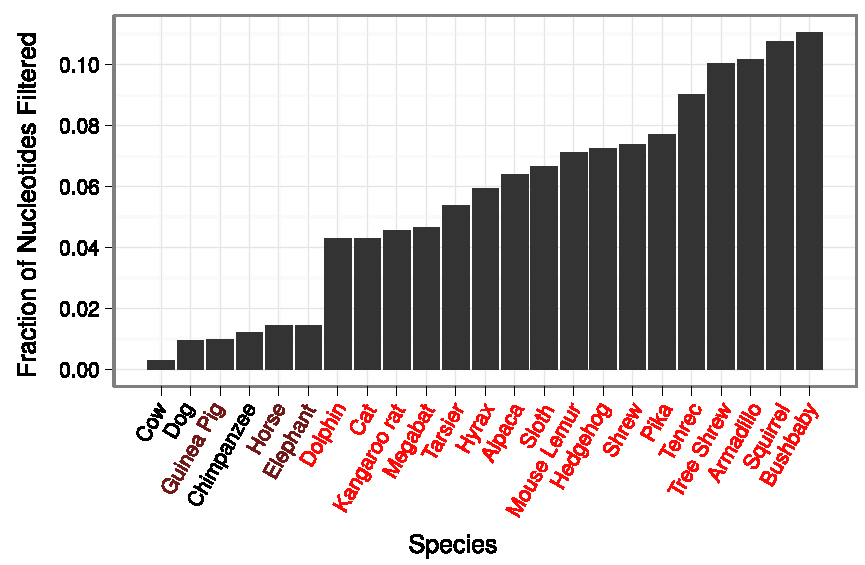
\includegraphics[scale=0.9]{Figs/qual_filter_hist.pdf}
\caption{}
\label{filtered_qual_bars}
\end{figure}

The above filtering scheme was applied to all coding sequences from
each species for which quality scores were available, which included
all of the species with \lcv genomes as well as five with
high-coverage genomes: chimpanzee, guinea pig, dog, horse, cow, and
elephant. (Note that guinea pig and elephant genomes were originally
sequenced at low 2x coverage for the \ac{mgp}, but they have since
undergone additional sequencing to produce high-coverage 7x
assemblies. These assemblies were used in \ens version 63 and thus in
the analysis described below.) The overall percentage of nucleotides
filtered from each genome is shown in Figure
\ref{filtered_qual_bars}. As expected, genomes with high-coverage
sequences contained fewer bases with low Phred scores, resulting in
1-2\% of nucleotides being filtered. The bulk of low-coverage genomes
resulted in 4-8\% of nucleotides being filtered, while five genomes
(bushbaby, squirrel, tree shrew, armadillo and tenrec) showed a
noticeably higher proportion of low-quality bases, with 9-11\%
nucleotides being filtered out. The distribution of filtered
nucleotide proportions confirmed the expectation that 5-15\% of
nucleotides would be filtered using a Phred score threshold of 25, and
the variation in filtered nucleotide proportions between different
species showed that despite the uniform 2x coverage of the \lcv
mammalian genomes, different assemblies varied widely in their
distributions of sequence quality scores within coding regions.

\subsection{Removing recent paralogs}
\label{sec_removing_paralogs}

As discussed in Section \ref{section_quantifying_paralogous}, the
inclusion of paralogous gene relationships in a large-scale analysis
of orthologous gene evolution may produce misleading signals of
adaptive evolution \citep{Lynch2000}, artifacts resulting from gene
conversion \citep{Casola2009}, and produce biases due to lineage-specific
family expansion, a process which is relatively common in mammalian
gene families \citep{Gu2002}. As a result, it has traditionally been
considered important to filter out recently-duplicated genes (e.g.,
genes duplicated after the whole-genome duplication event in the
vertebrate ancestor) in large-scale evolutionary analyses. Previous
genome-wide scans for positive selection involving six or fewer
mammalian genomes have either required strict one-to-one orthology
\citep{Clark2003,Nielsen2005} or allowed very limited numbers of
recent duplications in specific lineages \citep{Kosiol2008}. With
larger mammalian trees, however, the requirement of strict one-to-one
orthology becomes increasingly untenable: if gene duplications and
deletions occur randomly in time, then the probability of observing at
least one such event in a given gene family should increase linearly
with the amount of branch length covered by the tree. The requirement
of one-to-one orthology would result in fewer genes being available
for analysis as more species are incorporated into the analysis, which
is clearly an undesirable trend. As an alternative to ignoring genes
which do not satisfy the requirement of strict orthology, I developed
an approach, described below, for handling recently duplicated genes
by removing the more-divergent paralogous copy from the the gene tree.

%Before describing the method for duplications, it is worth making a
%point about gene deletions. Specifically, I note that gene deletions
%can complicate the branch-specific detection of positive selection,
%but they should not have a detrimental effect on tests for selection
%across the entire tree. The effect on branch-specific tests results
%from the merging of multiple ancestral branches into one. Take for
%example the inference of mutations along the evolutionary tree of
%human, chimpanzee and gorilla, which contains two internal nodes:
%$HC$, the human-chimpanzee ancestor, and $HCG$, the
%human-chimpanzee-gorilla ancestor. When sequences from all species are
%present, mutations can be separately identified as occurring along the
%branch from $HCG$ to $HC$ and along the branch from $HC$ to the human
%sequence, allowing for a test to differentiate between a signal of
%adaptive evolution in one branch or the other. For a gene which was
%deleted in chimpanzee those two branches become effectively merged
%into one, and mutations can only be inferred to have occurred between
%$HCG$ and the human sequence. The time-specificity of estimated
%evolutionary rates is thus reduced, and when the identity of the
%branch along which \syn and \nsyn mutations have occurred is important
%to a test for positive selection, this difference can complicate the
%interpretation of results. Acknowledging this effect,
%\citet{Kosiol2008} used a different set of orthology requirements for
%each branch-specific test for positive selection performed. When the
%test for positive selection does not depend on the identity of
%specific branches in the tree, however, a gene deletion would only
%serve to reduce the total amount of branch length available for
%inference. As long as the branch leading to the deleted species did
%not comprise a large portion of the total branch length, the effect of
%gene deletion on the results of tree-wide tests for selection should
%be minimal.

%Turning back to gene duplications, 
An additional complicating factor
in the current analysis was the concern that many of the apparent gene
duplications were actually artifacts of the annotation of \lcv
genomes. Each \lcv genome assembly is highly fragmented, meaning that
it contains many short sequence segments that were unable to be
assembled into chromosome-sized sequences due to missing sequence
data. Sometimes the exons of a gene spanned the boundaries of these
sequence segments, causing different parts of a gene to exist on
different segments. The \ens annotation pipeline was not designed to
merge gene annotations across different sequence segments, so each
part of a gene residing on multiple sequence segments would be
annotated as a separate shortened gene. These shortened genes would be
treated as independent proteins by the \cmp pipeline, likely being
placed at very similar positions in the gene tree due to each sequence
having been derived from a gene with a single correct evolutionary
position. While this result might not be detrimental to sitewise
analysis in itself (as each shortened gene might be correctly aligned
and provide useful information to the alignment), a number of factors,
including the low quality of genomic sequence and assembly within
these shortened genes, problems with aligning small fractions of a
gene against complete sequences, and the potential for incorrect
placement of fragmented sequences within the gene tree, made it
desirable to remove these shortened genes before estimating
evolutionary rates. These split genes could be effectively identified
by their shortened length.

Sequence divergence was the other criterion by which I selected which
paralogous copy of recently-duplicated genes to retain for
evolutionary analysis. A well-established theoretical model of
evolution after gene duplication predicts that one of the duplicate
copies retains the ancestral function (and its associated pattern of
evolutionary constraint) while the other duplicate experiences relaxed
constraint followed by either degradation or functional
diversification \citep{Han2009}. Thus, the least-diverged copy of a
recently duplicated gene should be the one most likely to have
retained the pattern of evolutionary constraint shared among the
mammalian species being examined in this study.

The protocol I implemented for filtering apparent paralogs used both
gene length and sequence divergence to identify which gene among a set
of apparent paralogous copies was most suitable to retain for sitewise
analysis. Gene length was used primarily to discriminate spuriously
shortened genes from true genes, and sequence divergence was used to
distinguish between more- and less-diverged paralogs. First, the mean
pairwise sequence distance was calculated between each putative
paralog and all other sequences in the gene tree, resulting in one
mean pairwise distance estimate per putative paralog (hereafter
referred to as the mean distance). For these distance calculations,
the stock \cmp codon alignments and the JC69 nucleotide model to
estimate distances. Second, the ratio of the sequence length of each
putative paralog to the mean sequence length across the tree
(hereafter referred to as the length ratio) was also calculated.

Genes were grouped by species within each gene tree, and any group of
2 or more genes was considered to be a set of putative paralogs
. Within each set of putative paralogs, a single gene was chosen to be
retained for evolutionary analysis based on three rules applied in the
following order: (1) if only one sequence had a length ratio above 0.5
and all others had a length ratio below 0.5, the longest sequence was
kept; (2) if at least one sequence yielded a mean distance below the
others, that sequence was kept; (3) if all mean distances were
identical then the longest sequence was kept, or if all mean distances
and length ratios were equal, an arbitrary choice was made.

\begin{figure}
\centering
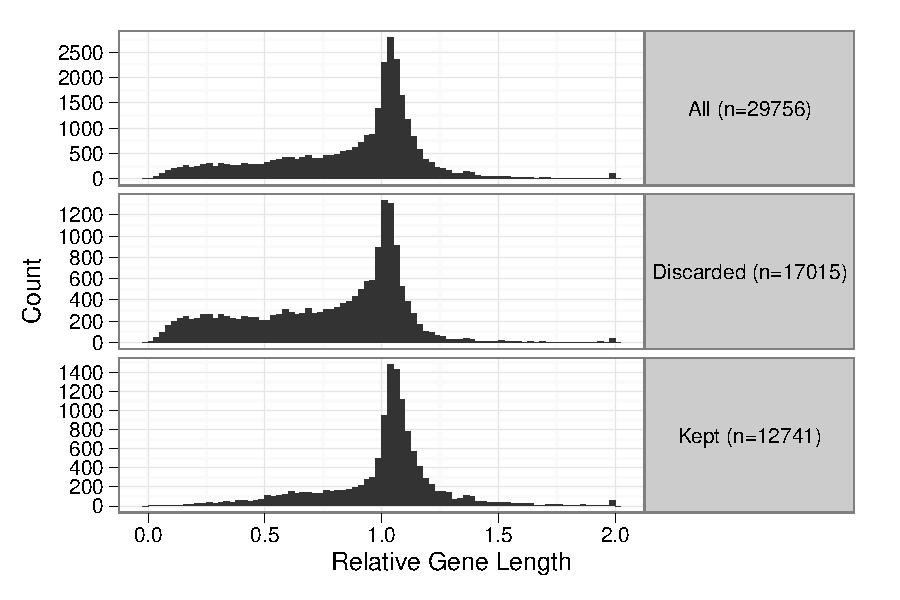
\includegraphics[scale=0.7]{Figs/filtered_paralogs_hist.pdf}
\caption{Length ratios of putative paralogs. The length ratio was
  calculated as the length of a putative paralogous copy divided by
  the mean length all sequences its corresponding gene
  tree. Putatively paralogous genes (top panel) were either discarded
  (middle panel) or kept (bottom panel) according to rules based on
  their length and mean sequence divergence from other aligned
  sequences, as described in the text.}
\label{filtered_paralogs_hist}
\end{figure}

These rules were applied to each of the 29,756 putative paralogs
contained within the 16,XYZ largely orthologous gene trees from the
previous chapter. Figure \ref{filtered_paralogs_hist} shows the
distributions of length ratios separately for the set of all putative
paralogs, those discarded from the alignments, and those kept for
subsequent analysis. The overall distribution of length ratios shows
that most putative paralogs had lengths similar to the mean length
across the gene tree (with a peak at or slightly above 1), but the
shape of the distribution was asymmetric, with a strong bias towards
shorter lengths. The filtering protocol effectively removed these
shortened genes, as evidenced by the strong enrichment of lower length
ratios in the distribution of discarded genes and the less skewed
distribution of length ratios in the set of XYZ kept paralogs.

\begin{figure}
\centering
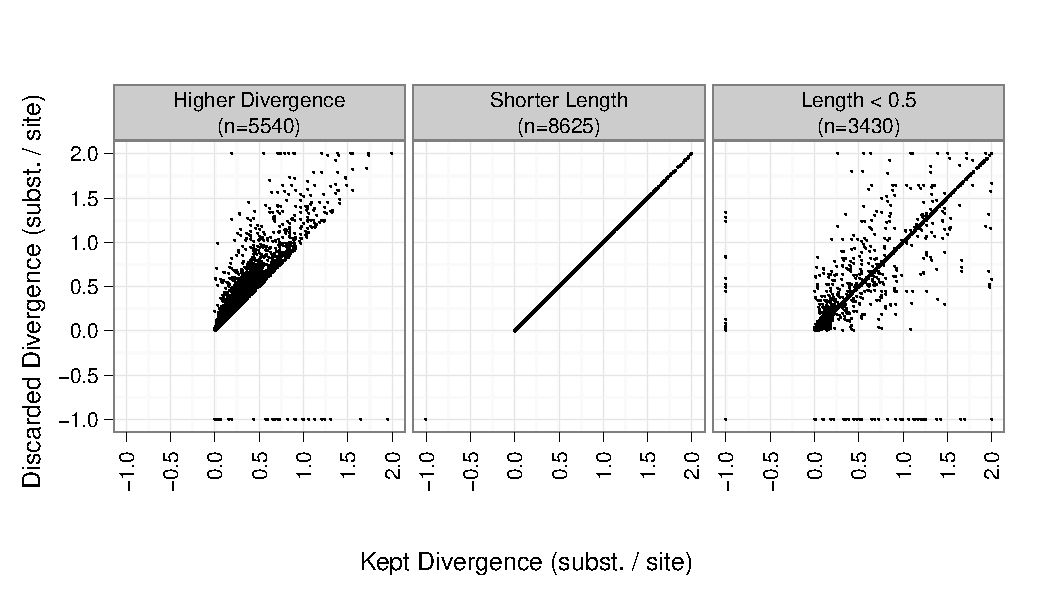
\includegraphics[scale=0.7]{Figs/filtered_paralogs_scatter.pdf}
\caption{Sequence divergence of kept and discarded putative
  paralogs. Each point represents a gene which was discarded from the
  tree for one of three reasons: it had more sequence divergence than
  the kept gene (\emph{Higher Divergence}; left panel), it had equal
  sequence divergence but shorter length than the kept gene
  (\emph{Shorter Length}; middle panel), or it had a gene length
  (relative to the mean across all sequences) of less than 0.5 while
  the kept copy had a relative length greater than 0.5 (\emph{Length
    $<$ 0.5}; right panel). Divergence was measured as the mean
  pairwise divergence between the gene and all other sequences in the
  tree, and a value of -1 was assigned to genes for which no reliable
  divergence estimate could be attained due to a lack of sufficient
  data)}
\label{filtered_paralogs_scatter}
\end{figure}

To better compare the characteristics of the discarded and kept genes,
a dmore detailed view of the results of the paralog filter is
presented in Figure \ref{filtered_paralogs_scatter}, showing a scatter
plot of the mean distance and length ratio of each discarded paralog
compared to that of the corresponding kept paralog. Figure
\ref{filtered_paralogs_scatter} is separated into panels according to
the rule used to discard the paralogous copy: the first panel
corresponds to rule (1), where genes with a length ratio below 0.5
were discarded; the second panel corresponds to rule (2), where genes
with higher mean distances were removed; the third panel corresponds
to rule (3), where all genes had equal mean distances and the longest
gene was kept (or, if all lengths were equal, an arbitrary choice was
made).

The first panel of Figure \ref{filtered_paralogs_scatter} shows that
genes discarded on the basis of having a very short length contained
sequence distances similar to the kept copies, as the highest density
is along the diagonal and there is no apparent bias for genes to lie
above or below the diagonal. This is in line with the expectationq
that these discarded genes were not truly paralogous copies, but
rather fragments of split genes resulting from unassembled sequence
segments. The second panel shows that when paralogous copies could be
differentiated by their mean distances, they tended to have low
average distances ($<$0.5 substitutions per nucleotide site) and only
a small difference between the kept and discarded copy (e.g., most of
the distribution is just above the diagonal, and few points are above
the dashed line with a slope of 2). Finally, the distribution of
length ratios and mean distances in the set of genes where length was
the discriminating factor (or where an arbitrary decision was made)
shows that most of these genes were mostly identical whether measured
by sequence distance or sequence length.

These results provided evidence that a sizeable fraction of recently
duplicated mammalian genes are identical or very similar to each
other: for roughly 30\% of putative paralogs, not enough time has
elapsed since the duplication event for a detectable amount of
sequence change to have occurred, and the choice between retaining one
copy or the other was essentially arbitrary. For the roughly 40\% of
putative paralogs where differences in mean distance could be
identified, these differences tended to be small, suggesting that
massive functional divergence of recent gene duplicates has not been a
common phenomenon in mammalian evolution. Nonetheless, this protocol
was designed to identify the least-diverged copy of a recently
duplicated gene, and for 40\% of putative paralogs the mean distance
to other sequences in the gene family allowed a sensible decision to
be made.

This was obviously not the most conservative approach to dealing with
recent duplications---one could instead remove all copies from a set
of putative paralogs, creating an apparent gene deletion in that
species, or simply ignore all gene families with any recent
duplications (e.g., require one-to-one orthology allowing for gene
deletions). The latter option would likely be overly conservative for
a mammal-wide analysis, but the former option may be appropriate for a
more conservative approach. As the main concern over the handling
duplicated genes has been that they may introduce a bias towards
elevated evolutionary rates, I marked the genes containing sets of
putative paralogs for further evaluation. Sitewise estimates from
these genes were excluded from the most conservatively-filtered
sitewise dataset and examined separately for excess signal of positive
selection (see Section \ref{section_sitewise_filtering})
%, and in the
%next chapter I examine whether using the more conservative approach of
%removing all paralogous copies from genes removed the signal of
%positive selection from a subset of genes (see Section
%\ref{section_genes_paralog_subset}).

\subsection{Identifying clusters of \nsyn substitutions}
\label{section_windows_clustered_subs}

After filtering for sequence quality and removing paralogous genes and
shortened gene fragments, PRANK was used to align the codon sequences
of each of the 16,477 mammalian gene trees. Manual analysis of a
number of these alignments revealed many short stretches of clearly
nonhomologous sequence in one species, often flanked by stretches of
perfect homology and often lying on the borders of exon junctions.
%An
%example of one such region is shown in Figure \ref{figure_TODO}. In
%this otherwise highly conserved region of the XYZ gene, a short
%20-codon stretch of the XYZ sequence appears to contain little
%homology to the sequences from other species.
These obviously erroneous stretches were likely due to mis-assembly of
a genomic region orf misidentification of exon boundaries within the
gene of one species. These errors were particularly concerning with
respect to the detection of positive selection, as the incorporation
of a stretch of apparently nonhomologous material into a sequence
alignment would produce many alignment columns with multiple
nucleotide differences per codon. As discussed in Section
\ref{sec_error_impact}, this type of error is particuarly prone to
cause false positives in the detection of positive selection.

I hypothesized that these stretches of \nhom sequence could be
identified by their impact on the pattern of substitutions within each
alignment. A stretch of \nhom aligned sequence would be expected to
produce a localized cluster of apparent synonymous and nonsynonymous
substitutions occurring along the branch between the sequence
containing the erroneous stretch and its ancestor. Because these
substitutions would be restricted to one terminal branch in the gene
tree and a region of the alignment limited to the length of the \nhom
stretch, a scan for clustered substitutions within the terminal
lineages of genes might be an effective way of identifying these
erroneous sequences.

Two factors could confound the effectiveness of using clustered
substitutions to identify regions of \nhom aligned sequence. First,
the length of the terminal branch leading to each species determines
how many lineage-specific substitutions would be expected to occur
within a window of a certain size. The terminal human branch, for
example, is very short, while the platypus branch is very long. Thus,
one would expect to observe many more lineage-specific substitutions
in platypus than in human for a given alignment window. In contrast, a
stretch of \nhom aligned sequence should introduce, on average, a
constant number of \nsyn and \syn substitutions into the branch
ancestral to the sequence in which it exists. For this reason it
should be more difficult to distinguish homologous from \nhom
stretches in species with long terminal lineages. On the other hand,
this trend should also serve to limit the negative impact of \nhom
stretches in those species on the detection of positive selection,
because the resulting elevation in \nsyn or \syn substitutions rates
would be less severe.

The second confounding factor is that \nsyn substitutions have been
shown to be significantly more clustered than expected by chance in a
number of genomic analyses of mammalian and insect genomes
\citep{Callahan2011,Bazykin2004,Wang2007}. Thus, a filter based on
clustered \nsyn substitutions may have a tendency to remove true
clusters of \nsyn substitutions from the dataset. The influence of
this factor may be evaluated by comparing clusters of substitutions in
terminal branches to those in internal branches: while both internal
and terminal branches of the mammalian tree should harbor similar
levels of truly clustered \nsyn and \syn substitutions, only the
terminal lineages should contain large clusters resulting from
stretches of aligned \nhom sequence.

I investigated the distributions of \nsyn and \syn substitutions
within windows of mammalian alignments by using \emph{codeml}
\citep{Yang2007PAML} under the M0 model (e.g., assuming one \omg for
all sites and all branches in the tree) to perform the marginal
reconstruction of ancestral sequences at internal nodes
\citep{Yang1995} and to identify the substitution events implied by
the reconstructed ancestral sequences of each gene alignment. Only
substitution events occurring between codons with high posterior
probabilities in the marginal ancestral reconstruction ($>0.9$) were
analyzed, and the location of each substitution event along the
alignment and within the gene tree was stored. This analysis was
performed on all gene trees, yielding a large database of confidently
inferred substitution events along internal and terminal branches of
the mammalian phylogenetic tree.

Counts of \syn and \nsyn substitutions along each branch were
collected for non-overlapping 15-codon alignment windows; the results
for a selection of species and internal nodes are shown in Figure
\ref{fig_wcs}, which plots the number of 15-codon windows containing a
given number of \nsyn and \syn substitutions for a selection of
terminal and internal nodes. The mean length of the branch ancestral
to the given node, indicated in parentheses after each node name, was
calculated from the set of branch lengths estimated by \emph{codeml}.

\begin{figure}
\centering 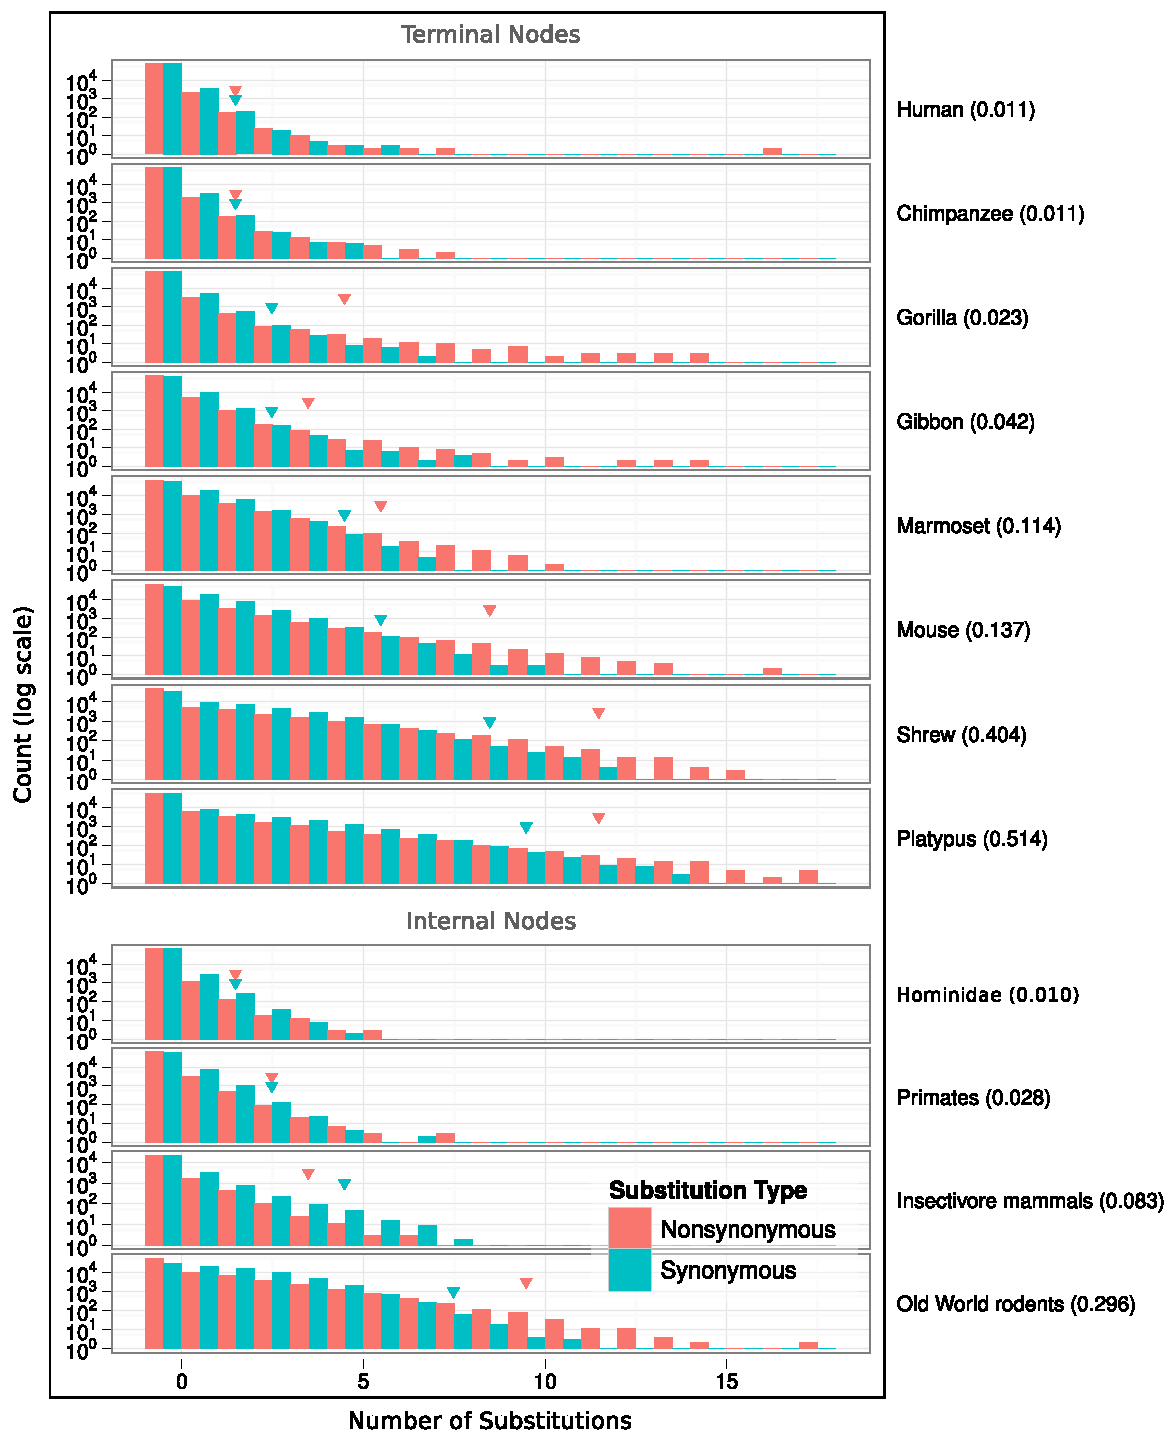
\includegraphics[scale=0.75]{Figs/wcs_15.pdf}
\caption{Counts of inferred \nsyn (red bars) and \syn (blue bars)
  substitutions in 15-codon windows along terminal and internal
  branches of the mammalian tree. The leftmost two bars correspond to
  windows with 0 substitutions, the next two bars correspond to
  windows with 1 substitution, and so on. Red and blue arrows indicate
  the number of \nsyn and \syn substitutions, respectively,
  corresponding to the 99.9\% percentile across all windows in that
  node.}
\label{fig_wcs}
\end{figure}

Figure \ref{fig_wcs} shows that the vast majority of 15-codon windows
in these alignments contained few substitutions (note that the y-axis
uses a logarithmic scale), but a long tail of \nsyn and \syn
substitutions were observed for some nodes. Comparing the counts of
\nsyn vs. \syn substitutions within the terminal nodes (Figure
\ref{fig_wcs}, top panel), a pattern is seen where the \nsyn counts
(red bars) are higher than \syn counts at 0 substitutions, lower than
\syn counts in the middle range of substitutions (1--5 substitutiosn),
and higher again in the higher range of substitutions ($>$5
substitutions). The pattern in the lower range is consistent with the
action of purifying selection on protein-coding regions, causing a
reduced number of windows with multiple \nsyn substitutions compared
to \syn substitutions. The excess of windows with large numbers of
\nsyn substitutions, on the other hand, runs against the pattern of
purifying selection; instead, it shows unexpectedly long clusters of
\nsyn substitutions to be a widespread feature of these mammalian
alignments. The red and blue triangles drawn in each plot mark the
number of substitutions below which 99.9\% of windows are contained;
the shift of the \nsyn markers to the right emphasizes the excess of
highly clustered \nsyn substitutions. Interestingly, human---which has
the highest quality and best annotated genome---does not show the same
level of excess seen in the other genomes analyzed.

Comparing the pattern seen for terminal nodes to those from internal
nodes provided further evidence for the presence of many stretches of
\nhom sequence within the mammalian alignments. For example, the
terminal gorilla node is roughly equivalent in average branch length
to the internal primates node ($0.023$ vs. $0.028$), but gorilla
contains windows with up to 14 \nsyn substitutions while primates
contain a maximum of 8. Looking at the \nsyn and \syn 99.9\%
quantiles, three of the four internal nodes had equal quantile
positions for \nsyn and \syn substitutions, but the rodent ancestral
node did not. This was an interesting difference, as the gene
annotations for most rodent genomes were likely derived from
alignments to mouse rather than human. In the case of discordant gene
annotations, the entire rodent clade would share an aligned \nhom
stretch, causing clustered substitutions to be inferred along the
internal rodent branch. This raised the possibility that the entire
rodent clade contains many misaligned \nhom stretches due to
differences in gene annotations between rodent and non-rodent species.

%This appeared to be the case for at least one gene: Figure
%\ref{fig_mouse_crap_aln} shows the region surrounding a 15-codon
%window with 11 apparent rodent \nsyn substitutions, likely the result
%of a difference in exon annotations between rodent and non-rodent
%genomes.

The end result of this analysis was the identification, for each
terminal node of the mammalian tree, windows with \nsyn substitution
counts above the top 0.1\% of 15-codon windows genome-wide; these
windows were considered potential stretches of \nhom aligned
sequence. Despite evidence that some internal nodes might also suffer
from this type of alignment artifact, most internal nodes were free
from an obvious excess of clustered \nsyn substitutions, so internal
nodes were excluded from this list. And although there is no way to
show that the 0.1\% threshold is the most appropriate one for
discriminating true from erroneous windows of clustered substitutions,
manual analysis of regions containing windows at a variety of
thresholds showed it to perform well.

In total, 30,XYZ \draft{numers are approximate, will fill in later}
windows containing potential stretches of \nhom aligned sequence were
identified across 3,XYZ genes, with XYZ genes containing at least 1
such window and XYZ genes containing greater than 10. The locations of
these windows were stored for later use in defining the most
conservatively-filtered sitewise dataset, and the impact of these
potentially \nhom windows on sitewise levels of positive selection is
described in Section \ref{section_stringent_filter}.

\section{Genome-wide analysis of sitewise selective pressures in mammals}

\subsection{Species groups for sitewise analysis}

% latex table generated in R 2.13.0 by xtable 1.5-6 package
% Thu Sep 15 11:19:59 2011
\begin{table}
\centering \footnotesize
\begin{tabular}{lrb{8cm}rr}
\toprule
 & \multicolumn{2}{c}{Species} & \multicolumn{2}{c}{Median dS} \\
\cmidrule(r){2-3} \cmidrule{4-5}
Name & Count & List & MPL & Total \\
  \midrule
\input{Tables/species_set_summary.txt}
\bottomrule
\end{tabular}
\caption{Species groups used for sitewise analysis by \ac{slr}. The
  median \acp{mpl} and the median total branch length are shown for
  each species group, taken from the \ngenes branch lengths estimated
  by \ac{slr} for each gene. MPL -- mean path length.}
\label{table_species_set_summary}
\end{table}

For each alignment of mammalin orthologs, SLR was run separately on 10
different sets of mammalian species to obtain sitewise estimates in a
variety of species groups. For each species group, sequences
corresponding to species within the group were extracted from the
whole mammalian alignment (along with the corresponding \subtr) and
input to SLR, which was run with its default parameters. If fewer than
two sequences were available for a given gene and species group, the
sitewise analysis was skipped for that group. The species included in
each group are listed in Table \ref{table_species_set_summary} alongside the
\ac{mpl} and total branch length of their subtrees estimated as the
median value across all 16xyz gene-wise dS branch length estimates
from SLR.

Three species groups (Glires, Primates, and Laurasiatheria) were
chosen because they represent the three mammalian superorders with the
greatest taxonomic representation in Ensembl, providing an opportunity
to compare the molecular evolutionary dynamics of three monophyletic
mammalian groups containing varying levels of divergence, diverse
biological characteristics, and a number of high-quality reference
genomes. A fourth parallel mammalian subclade, Atlantogenata,
consisting of sloth, armadillo, tenrec, elephant and hyrax, was also
included, but the monophyly of this group is still under debate
\citep{Murphy2007,Churakov2009} and it contains only one high-coverage
genome. As such, it was not considered a primary target for the
mammalian superorder analysis. The different mammalian superorders
contained a wide range of total branch lengths, with 0.83 for
Primates, 0.97 for Atlantogenata, 1.90 for Glires, and 2.16 for
Laurasiatheria. A slightly different ordering was found when measuring
the trees by \ac{mpl}, with Glires having a significantly higher
\ac{mpl} (0.40) than the other groups despite having fewer species and
a lower total branch length than Laurasiatheria. This reflected the
higher neutral evolutionary rate in the Glires group, a
well-documented feature of rodent evolution likely resulting from
their long-term shorter generation time, which has been strongly
correlated with higher neutral evolutionary rates
\citep{Nikolaev2007,Smith2008}.

Two larger species groups, Eutheria and Mammalia, were chosen for the
purpose of measuring average sitewise selective pressures across
mammals as a whole. The Eutheria group consists of the union of the
mammalian superorder groups plus armadillo, and the Mammalian group
adds opossum, platypus, and wallaby for a total of 38 species. The
median total branch lengths for Mammalia and Eutheria were 8.21 and
6.43, respectively, and the \ac{mpl}s were 0.67 and 0.35.

Finally, to evaluate the impact of species choice and branch length on
the results of the \sw analysis, four additional ``sparse'' species
groups were created for comparison to the main groups of interest. The
species in the Sparse Glires group were chosen to create a group with
species from the Glires group but having a lower overall branch
length; the Sparse Mammals group was created with a similar aim,
created by selecting one species (preferably with a high-coverage
genome) from each major mammalian branch, greatly reducing the total
branch length covered but maintaining a similar evolutionary depth and
distribution of major branches within the species tree. The HQ Mammals
group was similar to the Sparse Mammals group, but elephant and the
deeper mammalian lineages were omitted (e.g., wallaby, platypus,
armadillo) in favor of only the high-coverage Eutherian genomes (e.g.,
chimpanzee, cow, horse, macaque, pig, rat). Finally, the HMRD group
consisted of human, mouse, rat, dog, and represented the type of
phylogenetic tree that was commonly analyzed early in the last decade
when only a few mammalian genome sequences were available. The HMRD
group was comparable to Primates and Atlantogenata in total branch
length, while HQ Mammals and Sparse Glires were more similar to
Glires.

\subsection{Evaluation of the bulk distributions and the design of a filtering approach}
\label{section_sitewise_filtering}

Sitewise data were collected from SLR and stored in a database for
storage and further analysis. The Mammals group, containing the most
branch length of all the datasets and representing the entire set of
aligned sequences, and the Primates group, containing the lowest
overall branch length, were used as representative species groups to
perform quality-control checks on the \sw data and to guide the
curation of filtered \sw datasets for each species group.

Some amount of filtering is usually necessary in genomic analyses, and
the situation is especially delicate in a scan for positive selection,
since non-biological artifacts often appear to represent elevated
evolutionary rates
\citep{MarkovaRaina2011,Schneider2009,Mallick2009}. To balance the
desire to maintain as much real data as possible with the concern that
a methodological bias may influence the results, two datastes were
generated by processing \sw data separately with two filters: a
relaxed filter, designed to retain much of the data while filtering
out the most obviously low-quality sites, and a conservative filter,
designed to remove a wider set of sites and genes that showed evidence
for potential errors or biases.

\bbfig
\centering
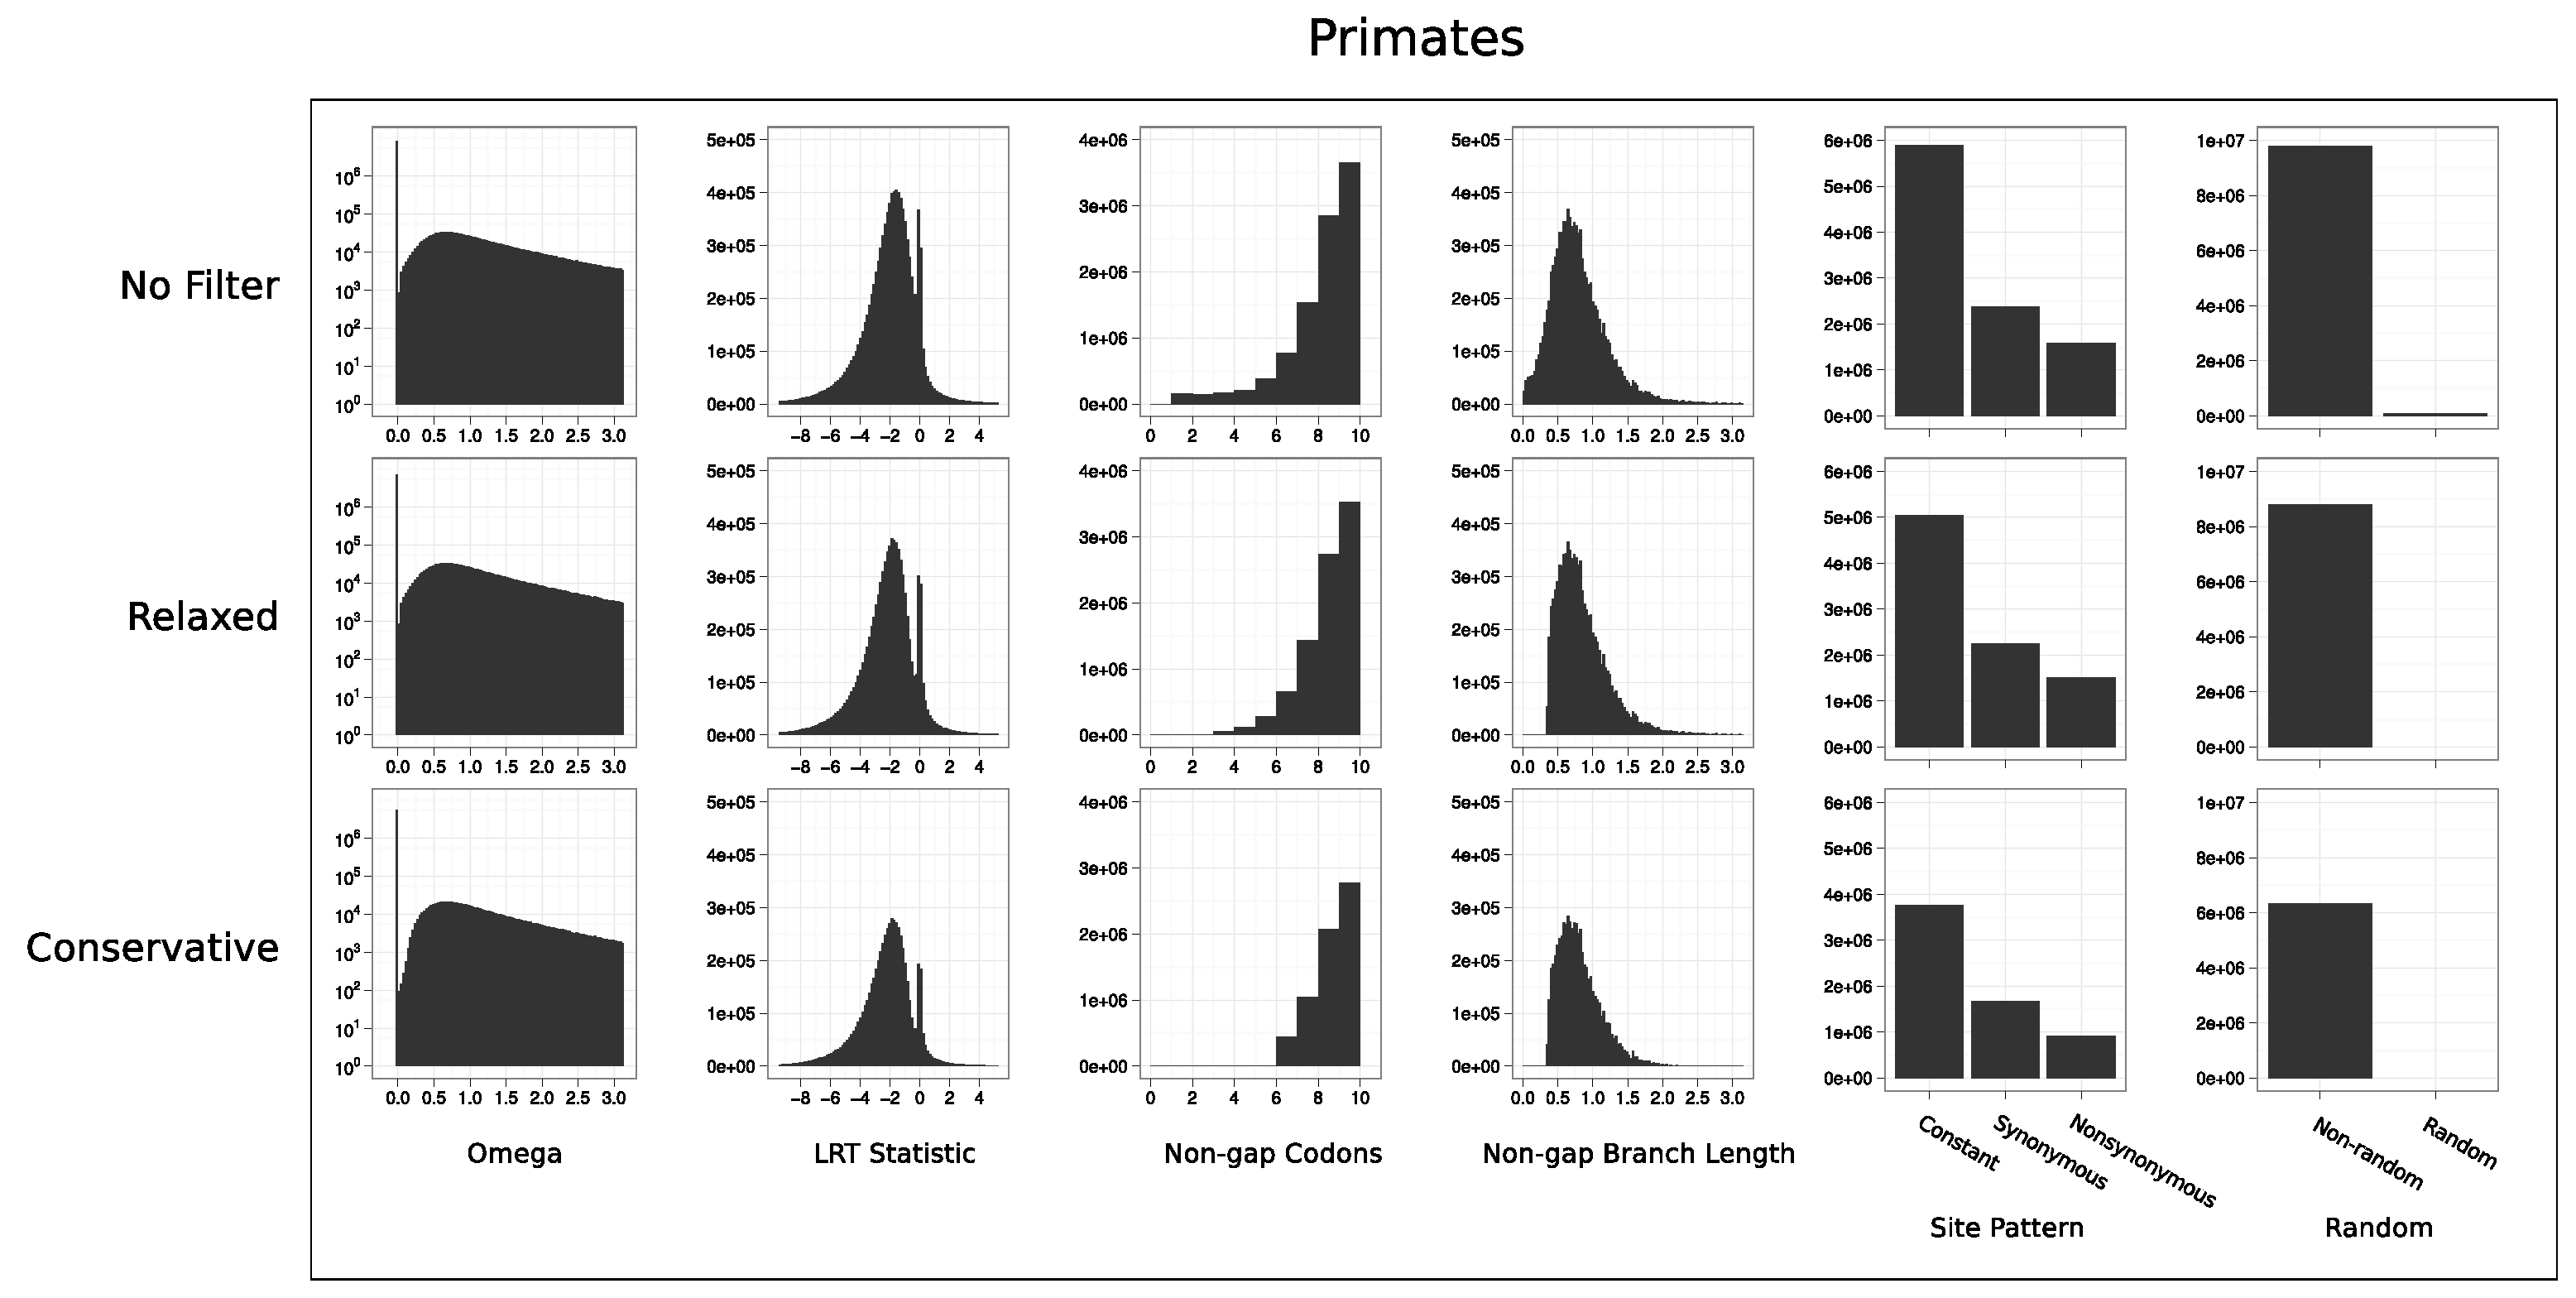
\includegraphics[scale=0.42]{Figs/qc_hist_primates.pdf}
\caption{Distributions of sitewise values for the Primates species
  group, showing the raw data (top row) and the result of applying the
  relaxed (middle row) and conservative (bottom row) filters.}
\label{fig_qc_hist_primates}
\eefig

\bbfig
\centering
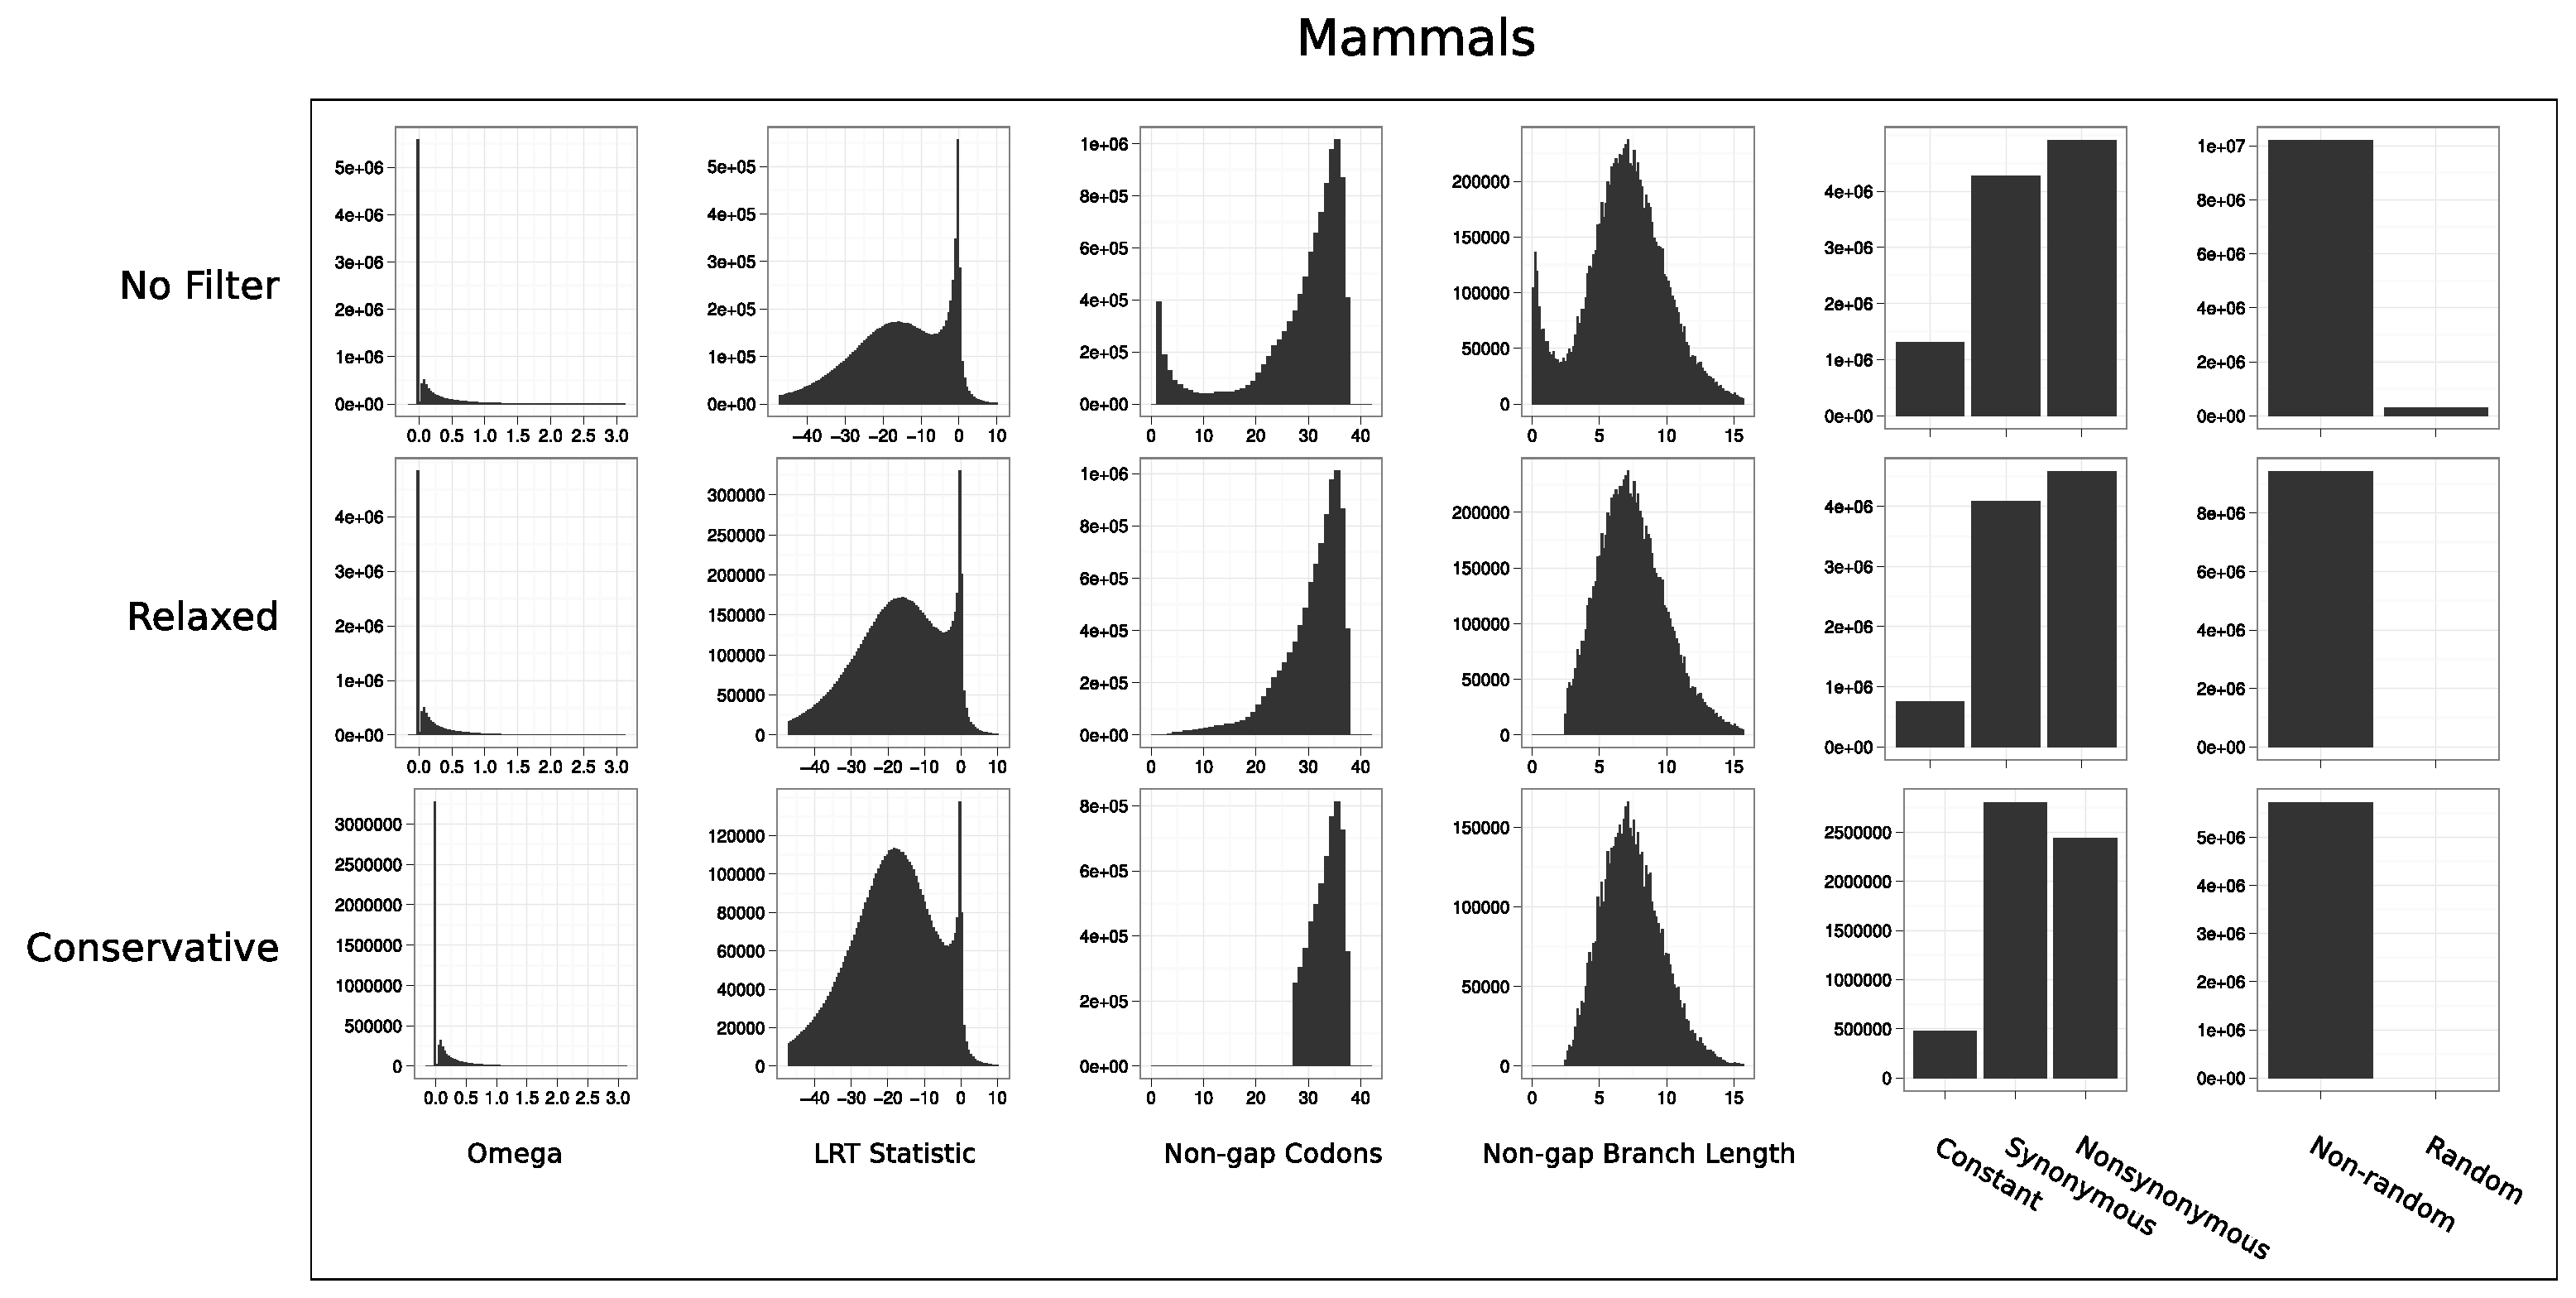
\includegraphics[scale=0.42]{Figs/qc_hist_mammals.pdf}
\caption{Distributions of sitewise values for the Mammals species
  group, showing the raw data (top row) and the result of applying the
  relaxed (middle row) and conservative (bottom row) filters.}
\label{fig_qc_hist_mammals}
\eefig
 
I first examined the overall distributions of \omg estimates and \sw
LRT statistics from SLR. Figures \ref{fig_qc_hist_primates} and
\ref{fig_qc_hist_mammals} show the distributions of six sitewise values
for each group of species: two continuous values and two categorical
values output by \ac{slr} (Omega, Signed LRT, Site Pattern and Random)
and two values calculated from the codon alignment (\Ngap Codons and
\Ngap Branch Length). \Ngap Codons is a count of the number of \ngap
codons in each alignment columnn, and the \Ngap Branch Length value
represents the total branch length connecting all non-gap sequences
(using the gene-wide branch lengths optimized by SLR).

A prominent feature of the distribution of \omg values for the
unfiltered Mammals data, shown in the top row of Figure
\ref{fig_qc_hist_mammals}, was the large number of sites with a
zero value for \omgml, the \ac{ml} point estimate of \omg. Further
inspection of the data revealed that all \omgml$=0$ sites contained
either \syn or constant site patterns. Furthermore, all sites with
constant patterns (and nearly all sites with \syn patterns) yielded a
\omgml estimate of zero. Intuitively, an estimate of zero for \syn
sites is appropriate, as the lack of any \nsyn substitutions
throughout the tree would provide no evidence for a \nsyn substitution
rate of greater than zero. For constant sites the case is less clear,
because no data regarding the rate of either \syn or \nsyn
substitutions exists in the alignment column. However, given SLR's
assumption of a constant \syn substitution rate throughout each gene
\citep{Massingham2005}, the \omg value which maximizes the likelihood
of observing zero substitutions is zero, since that value minimizes
both the \nsyn and the total substitution rate.

It is not evident from Figure \ref{fig_qc_hist_mammals}, but a small
proportion (ca. 0.2\%) of sites containing \syn site patterns resulted
in \ml estimates greater than zero. Analysis of the alignment columns
corresponding to these sites showed them all to include synonymous
codons coding for serine or arginine which are separated by multiple
nucleotide differences. Under the mechanistic codon model implemented
by \ac{slr}, which does not allow for multiple simultaneous nucleotide
changes, inferring an evolutionary path between these
multiply-substituted codons required the inference of multiple \nsyn
substitutions to reach one codon from the other. This produced a \nsyn
substitution rate of greater than zero for a site with a \syn site
pattern. The existence of multiply-substituted codons in alignments
has been previously reported \citep{Averof2000,Whelan2004}, and
empirical results have supported the notion that codon models that
allow for multiple simultaneous nucleotide changes better describe
evolution than those that do not \citep{Kosiol2007}. However, the very
low proportion of synonymous sites requiring nonzero \nsyn
substitution rates suggested that the impact of these effects on the
current dataset was minimal; this is likely due to the relatively
short branch lengths separating the nodes of the mammalian tree,
making it less probable that codons with multiple substitutions
(whether the result of simultaneous multiple nucleotide changes or
successive single changes) would be observed \citep{Kosiol2007}.

The distributions of the \Ngap Codons and \Ngap Branch Length values
in the unfiltered row of Figure \ref{fig_qc_hist_mammals} showed that
most alignment columns contained sequence data from many species (with
\Ngap Codons peaking at 36 and \Ngap Branch Length peaking at around 8
substitutions per site), but a noticeable portion contained only a few
non-gap sequences. If the alignment columns with low \ngap codon
counts represented accurate evolutionary histories, then the observed
excess of highly-gapped sites might be taken as an indication that
insertion events in terminal lineages or recent ancestral lineages
were prominent enough throughout mammalian evolution to leave a
noticeable signature of sites with very low non-gap codon
counts. Given the many possible sources of error in the annotation and
alignment of these sequences, however, a more likely scenario was that
sites with low codon counts and low branch lengths came from stretches
of sequence which only exist in a few species as a result of
annotation or alignment error. As a result, these sites might be
expected to show a higher probability of being nonhomologous and
showing spurious signals of positive selection. This would make such
sites prime candidates for filtering out prior to analysis.

\begin{table}
\centering \footnotesize
\begin{tabular}{lrrrrrrrrrr}
\toprule
 & BL & \multicolumn{3}{c}{Nongap BL} & \multicolumn{3}{c}{Nongap Codons} & \multicolumn{2}{c}{\omgml, \%} &  \\
\cmidrule(r){3-5} \cmidrule(r){6-8} \cmidrule(r){9-10}
 & Quantile & 25\% & 50\% & 75\% & 25\% & 50\% & 75\% & $< 1$ & $> 1$ & \psfive, \% \\
  \midrule
\input{Tables/bl_pos_sel_breakdown.txt}
\bottomrule
\end{tabular}
\caption{Proportions of sites with evidence for purifying and positive
  selection in the Mammalia and Primates datasets broken down by \ngap
  branch length. Sites were separated into 10 equally-sized bins of
  \ngap branch length and the sites within each bin were summarized by
  the $25^{th}$, $50^{th}$ and $75^{th}$ percentiles of \ngap branch
  length (BL) and \ngap codons, the percentage of sites with \omg
  estimated below or above 1, and the percentage of sites classified
  as positively-selected codons (PSCs) at a nominal 5\%
  FPR. BL--branch length; PSC--positively selected codons.}
\label{table_bl_pos_sel_breakdown}
\end{table}

To test the hypothesis that sites with few \ngap sequences would be
less reliable for analysis than other sites, I split the \sw estimates
from the Mammals and Primates groups into ten equally-sized bins of
\ngap branch length. Sites within each bin were summarized by
calculating the percentage of sites with \omgml less than or greater
than 1, as well as the percentage of sites showing evidence for
positive selection at a nominal 5\% \ac{fpr}, hereafter referred to as
\acp{psc}. The results of this analysis are presented in Table
\ref{table_bl_pos_sel_breakdown}. The lowest bin was a clear outlier
in the Mammals data, with nearly 17\% of sites having \omgml$>1$ and
2\% of sites being \acp{psc}. The other 9 bins with greater \ngap
branch lengths showed fewer sites with \omg~$>1$ and less evidence for
positive selection; within those 9 bins, a pattern of gradual increase
in the proportion of sites with {{\omgml$>1$}} and \acp{psc} was observed
at progressively higher \ngap branch lengths. The increase in evidence
for positive selection with increasing \ngap branch length could be
explained by genes with higher overall \dnds ratios (and presumably
more \acp{psc}) having higher branch lengths due to the increased rate
of \nsyn substitution. Overall, the pattern observed for the Mammals
data was consistent with the prediction that sites with few \ngap
sequences were not consistent with the general pattern of \sw data. In
terms of choosing an appropriate threshold on which to filter, Table
\ref{table_bl_pos_sel_breakdown} indicated that removing sites with
the lowest 10\% of \ngap branch length would remove most of the
apparently anomalous sites.

Table \ref{table_bl_pos_sel_breakdown} showed a similar trend for the
Primates dataset, although the distinction between the lowest bin and
the rest of the dataset was less obvious. The percentage of \acp{psc}
in the lowest decile was only slightly higher than in the next-highest
decile, and the proportion of sites with \omgml$>1$ was lower than in
all other bins. Thus, despite weaker evidence in the Primates data for
the anomalous nature of sites with few \ngap sequences, it still
appeared that filtering sites in the bottom 10\% bin would improve the
overall quality and consistency of the data.

Turning back to the bulk distributions in Figure
\ref{qc_hist_mammals_primates}, two other criteria were used to target
sites for removal before analysis. First, the rightmost panels of
Figures \ref{fig_qc_hist_mammals} and \ref{fig_qc_hist_primates}
depict a small set of sites designated as ``random''. These sites were
flagged by SLR as having a site pattern not significantly different
from random \citep{Massingham2005}, and they were also targeted for
removal before analysis of the global distribution. Second, all sites
with fewer than four \ngap sequences were removed. This was done to
avoid analyzing sites with very few sequences which were not within
the bottom 10\% of sites by \ngap branchlength.

At this point, all of the criteria used to define the relaxed filter
have been described: \ngap branch lengths, random flags, and the
number of \ngap sequences at each site.
%Table
%\ref{table_filtering_summary} summarizes the filtering criteria used,
%and 
The middle rows of Figures \ref{fig_qc_hist_primates} and
\ref{fig_qc_hist_mammals} show the summary distributions resulting
from applying the relaxed filter to the Mammals and Primates sitewise
data.

Three additional criteria were added to create the more conservative
filtered dataset. First, the threshold on \ngap sequence counts was
increased: all sites with a \ngap codon count below 75\% of the
maximum \ngap count for that species group were removed. Second, sites
and genes containing windows of clsutered \nsyn substitutions (as
identified in Section \ref{section_windows_clustered_subs}) were
removed: all sites overlapping the 23,116 15-codon windows with excess
\nsyn substitutions (using the 99.9\% quantile based definition of
excess substitutions from Section
\ref{section_windows_clustered_subs}) were masked out, and 819 genes
with greater than 10\% of sites covered by windows with excess \nsyn
substitutions were removed. Finally, the 3,333 genes which contained
more than 2 sets of putative paralogs were excluded.

As with the relaxed filter
%, the parameters of the conservative filter
%are listed in Table \ref{table_filtering_summary} and 
the result of
applying the conservative filter to the Primates and Mammals datasets is shown in
the bottom rows of Figures \ref{fig_qc_hist_primates} and
\ref{fig_qc_hist_mammals}. Comparing between the distributions in the three rows of Figure
\ref{fig_qc_hist_mammals}, the most prominent effect of the two
filters on the bulk distributions in was the removal of the excess of
sites with low non-gap branch lengths and non-gap codon counts. The
distributions of \omgml estimates and LRT statistics were
qualitatively unchanged unchanged, indicating that the overall
characteristics of the dataset were not significantly altered by this
filter.

Tables \ref{table_filter_summaries_1} and
\ref{table_filter_summaries_2} provide a quantitative summary of the
Mammals and Primates datasets before and after applying the two
filters. Also shown is the subset of sites overlapping with Pfam
domain annotations collected from \ens; as most Pfam domains represent
well-folded protein modules \citep{Finn2010}, the set of
Pfam-annotated sites were expected to exhibit stronger purifying
selection and be less prone to insertions or deletions and alignment
error. The rows labeled in parentheses summarize the set of sites
which were removed during the creation of the conservatively-filtered
dataset, either due to overlap with a window of clustered
substitutions (Clusters) or from being within a gene that contained
more than 2 recent duplications (Paralogs).

The columns in Table \ref{table_filter_summaries_1} show various
summary statistics of each \sw dataset including the number of sites,
the proportions of different site patterns, and the proportions of
purifying and positive selection based on \omgml estimates from
\ac{slr}. Table \ref{table_filter_summaries_2} provides the number and
proportion of identified \acp{psc} (columns under the heading
``Positively Selected Sites'') as well as the breakdown of sites into
purifying, neutral, and positively-selected at two different \ac{fpr}
thresholds (columns under the headings ``\chisqlt{0.1}'' and
``\chisqlt{0.05}'').

These views make clear the impact of extensive filtering on the
genome-wide levels of positive and purifying selection observed in the
data. The unfiltered data from the Primates group contained 9.07\% of
sites with \omgml~$>1$, and 0.59\% of sites were \acp{psc} at a
nominal 5\% \ac{fpr}; the evidence for positive selection was reduced
in the conservatively-filtered data, showing 7.87\% sites with
\omgml~$>1$ and 0.41\% \acp{psc}. An even stronger effect of filtering
was seen for the Mammals data, with \omgml~$>1.5$ being reduced from
5.71 to 2.73 between the unfiltered and conservatively-filtered
datasets, and the percentage of \acp{psc} reduced from 0.72\% to
0.35\%. The rows representing two sets of sites which were removed
during the conservative filtering process showed higher signals of
positive selection than the unfiltered data, suggesting that these two
filtering steps were at least somewhat effective in removing
potentially anomalous or untrustworthy sites from the dataset. For
sites removed from being within clusters of \nsyn substitutions, the
enrichment for signals of positive selection was clear: in Primates,
18.28\% of sites yielded \omgml~$>1$, and 1.47\% of sites were
\acp{psc} at a 5\% \ac{fpr} threshold, more than three times the
proportion of \acp{psc} seen in the conservatively-filtered
dataset. Sites removed as a result of being within genes containing
recent duplications showed less of a signal for positive selection,
but the proportions of \acp{psc} and sites with \omgml~$>1$ were still
above those seen in either the relaxed or conservatively filtered
datasets for both Mammals and Primates. Thus, genes that have
experienced many recent duplications in mammals contained higher
levels of positive selection even after the most-divergent paralogous
copies were removed.

\begin{landscape}
\begin{table}
\scriptsize{
\centering
\begin{tabular}{lllrrrrrrrrrrrrr}
\toprule
 &  & &  \multicolumn{3}{c}{Site Pattern, \%} & Med. & 
  \multicolumn{3}{c}{Nongap BL} & \multicolumn{2}{c}{\omgml} &
\multicolumn{4}{c}{\omgml Below / Above, \%} \\
\cmidrule(r){4-6} \cmidrule(r){8-10} \cmidrule(r){11-12} \cmidrule(r){13-16}
Name & Filter & Sites & Const. & Syn. & Nsyn. & Codons & Med. & Mean & SD & Mean & SD &
$< 0.5$ & $< 1$ & $> 1$ & $> 1.5$ \\
  \midrule
\input{Tables/filter_summaries_1.txt}
\bottomrule
\end{tabular}
\caption{\scriptsize Summary statistics of \sw estimates for Mammals and Primates
  data with various filters applied. Rows labeled (Clusters) and
  (Paralogs) contain sites excluded by the Conservative
  filter. Columns under the ``\omgml Below / Above'' heading measure
  the percentage of sites with \omgml below or above the indicated
  value. Med.---median, Const.---constant, Syn.---\syn, Nsyn.---\nsyn,
  BL---branch length. \label{table_filter_summaries_1}
}

\hspace{.2in}

\centering
\begin{tabular}{llrrrrrrrrrrrrrrrrrrrrr}
\toprule
 & & \multicolumn{8}{c}{Positively Selected Sites (\%)} &
\multicolumn{3}{c}{\chisqlt{0.1}, \%} &
\multicolumn{3}{c}{\chisqlt{0.05}, \%} \\
\cmidrule(r){3-10} \cmidrule(r){7-10} \cmidrule(r){11-13} \cmidrule(r){14-16}
Name & Filter & 
  \multicolumn{2}{c}{\chisqlt{0.1}} & \multicolumn{2}{c}{\chisqlt{0.05}} &
  \multicolumn{2}{c}{\chisqlt{0.01}}& \multicolumn{2}{c}{\bhfdr{0.05}} &
  Neg. & Neut. & Pos. & Neg. & Neut. & Pos. \\
%\cmidrule(r){2-3} \cmidrule(r){4-5} \cmidrule(r){6-7} \cmidrule(r){8-9}
\midrule
\input{Tables/filter_summaries_2.txt}
\bottomrule
\end{tabular}
\caption{\scriptsize Proportions of sites subject to positive, purifying and
  neutral selection at various \slrt thresholds for Mammals and
  Primates data with varous filters applied. The Benjamini-Hochberg
  method \citep{Benjamini1995} was used to identify the \slrt
  threshold at which FDR$<$0.05. For columns under the headings
  ``\chisqlt{0.1}, \%'' and ``\chisqlt{0.05}, \%'', Pos. and Neg. are
  the percentage of sites with significant evidence for positive and
  negative selection, respectively, and Neut. is the percentage of
  ``neutral'' sites not showing significant evidence for non-neutral
  selection.}
\label{table_filter_summaries_2}
}
\end{table}
\end{landscape}

\subsection{The global distribution of sitewise selective pressures in mammals}

\begin{figure}
\centering 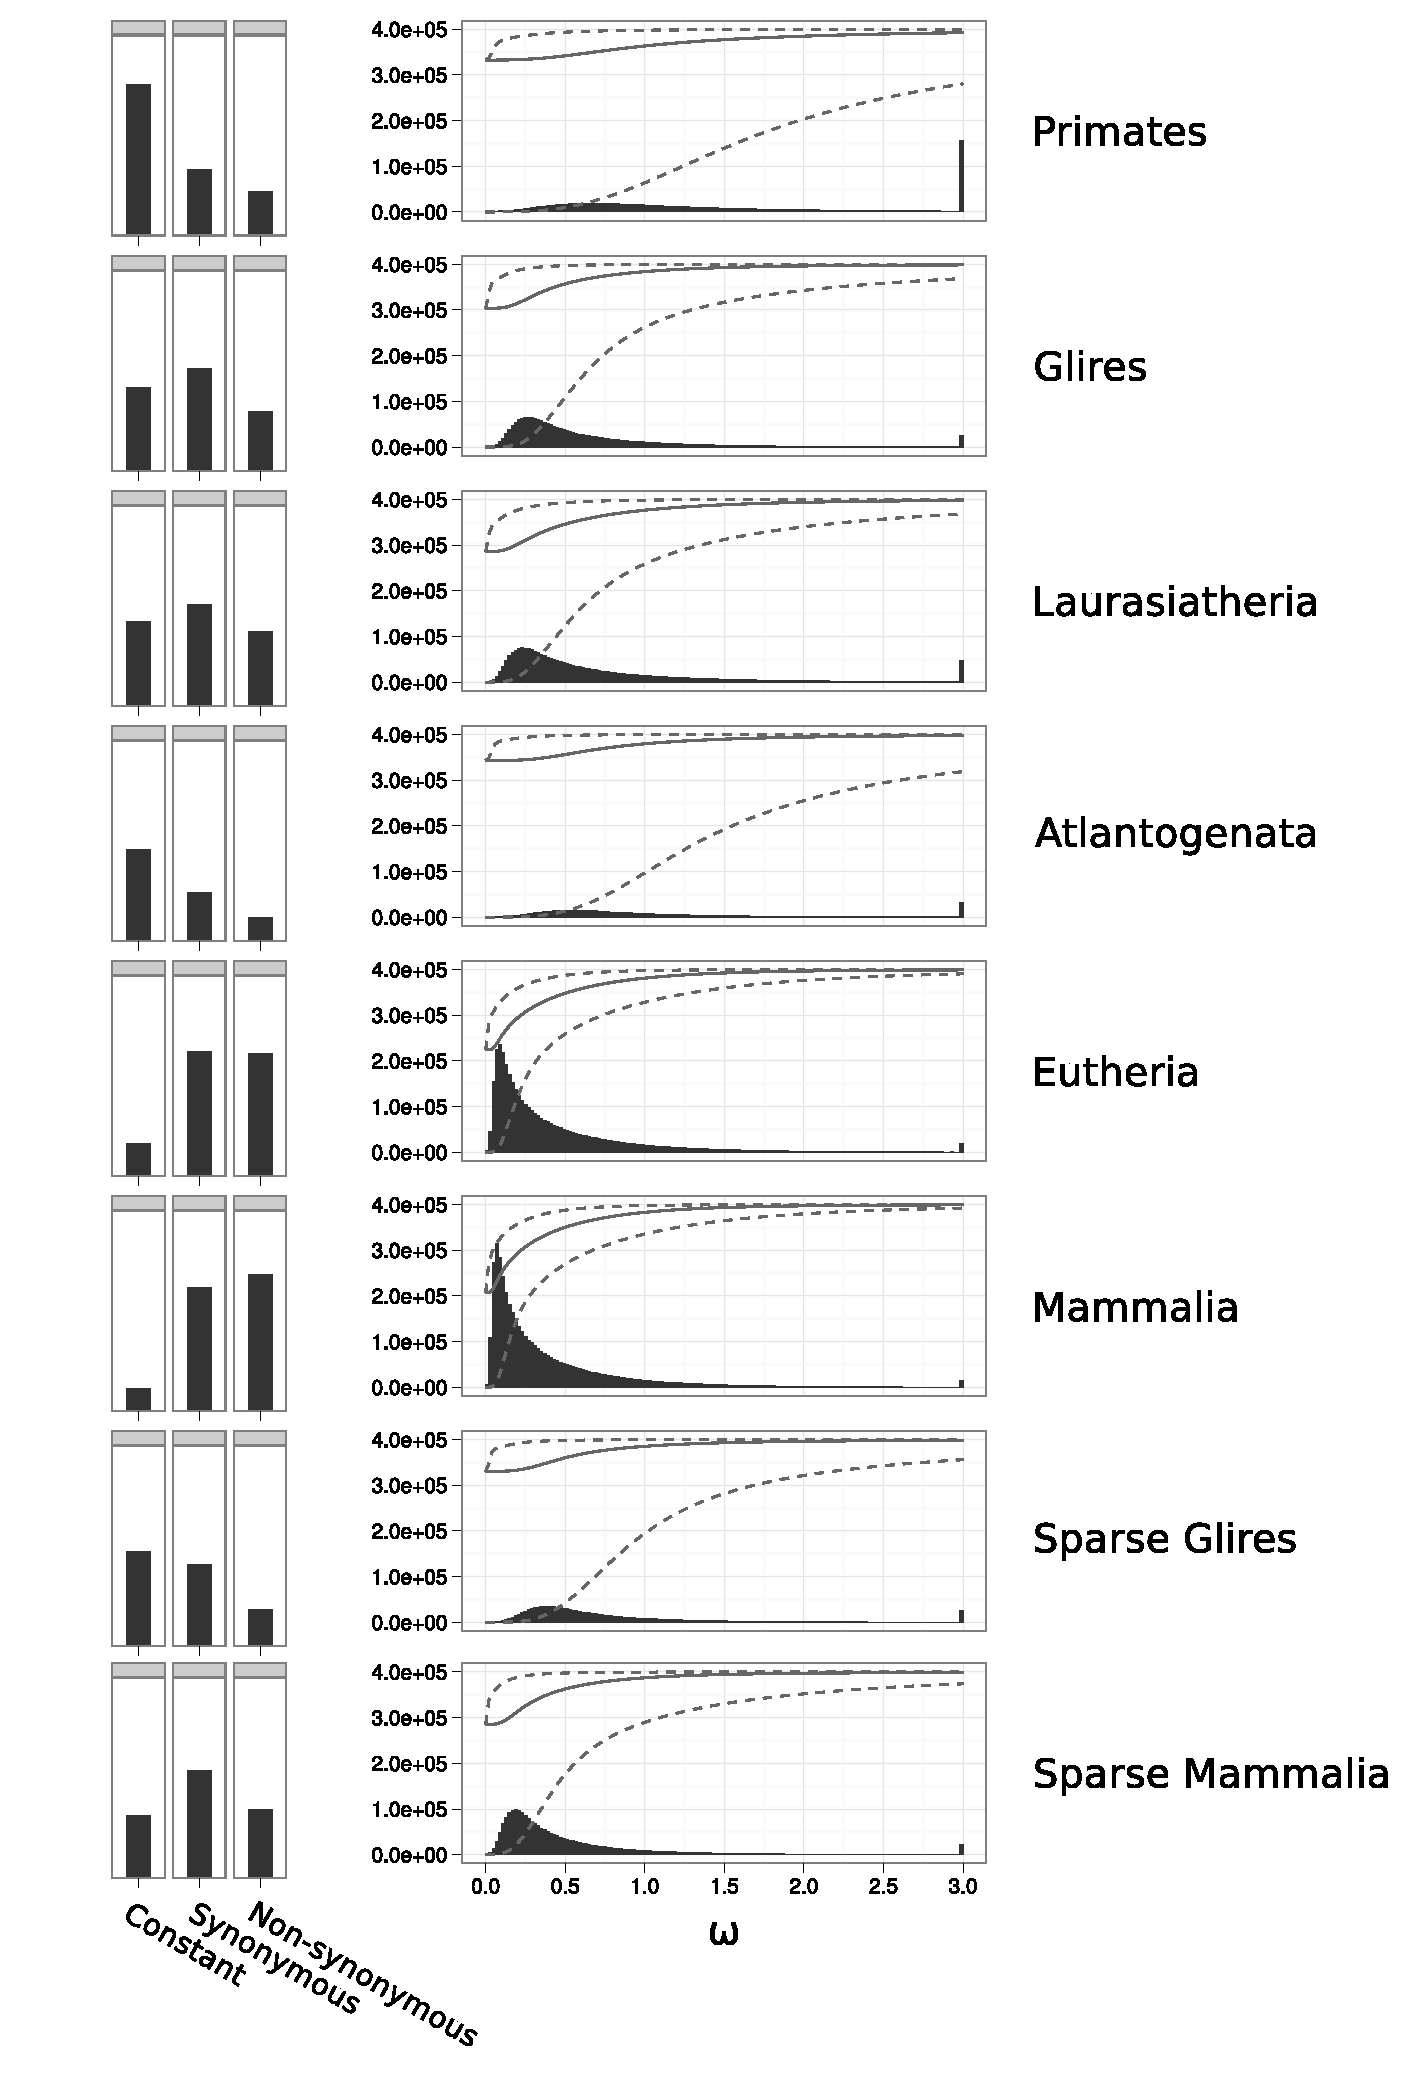
\includegraphics[scale=0.42]{Figs/global_distributions.pdf}
\caption{\scriptsize Global distributions of site patterns and \omg
  estimates for ten species groups. Left panels: bars represent the
  number of sites showing constant, synonymous, and non-synonymous
  patterns. Note, the y-axis is held constant between rows. Right
  panels: bars represent histograms of \omgml estimates for sites
  where \omgml$>0$. Sites with \omgml$>3$ are counted in the bin at
  \omgml$=3$. A solid line is drawn showing the cumulative
  distribution of \omgml, and dashed lines are drawn above and below
  the solid line showing the cumulative distributions of the lower and
  upper bounds, respectively, of the 95\% confidence interval
  associated with each \sw estimate.}
\label{fig_global_distributions}
\end{figure}

To produce high-confidence \sw estimates across the ten chosen species
groups, sitewise data from each species group were processed with the
conservative filter as described above. The resulting global
distributions of site patterns, sitewise \omgml estimates, and 95\%
confidence intervals are shown in Figure
\ref{fig_global_distributions}. The left panel in each row plots the
number of sites with constant, \syn, and \nsyn patterns; all sites
with \omgml$=0$ had constant or \syn patterns, and all sites with
\omgml$>0$ had \nsyn patterns. The right panel in each row shows the
distributions of \omgml for sites which contained a \nsyn site
pattern.

\subsubsection{Site patterns and \omgml values reveal the prevalence of purifying selection in mammalian proteins}

The site pattern counts in Figure \ref{fig_global_distributions}
showed that the branch length of each species group had a strong
effect on the overall composition of the sitewise data. Groups
covering little branch length, such as Primates and Atlantogenata,
contained mostly constant sites, while groups covering a large amount
of branch length, such as Eutheria and Mammals, contained few constant
sites and roughly equal proportions of sites with \syn and \nsyn site
patterns. Comparing the Glires and Mammals data with their
corresponding ``sparse'' datasets confirmed that this trend was
largely due to branch length as opposed to biological factors: the
Sparse Glires data, for example, yielded a smaller proportion of \nsyn
sites and a greater proportion of constant sites than the Glires data
(17.41\% versus 24.08\% for \nsyn sites, 44.21\% versus 33.98\% for
constant sites).

The distributions of \omgml estimates are shown in Figure
\ref{global_distributions} as a series of histograms showing the
\omgml density (for \nz values of \omgml only) and a series of solid
lines showing the cumulative \omgml density (representing all values);
the lower and upper dashed lines show the cumulative density of the
lower and upper 95\% confidence interval resulting from each \sw
estimate. From these distributions, it is clear that the majority of
protein-coding sites have evolved under purifying selection in
mammals, a fact which is most easily seen in the larger species
groups. The Mammalia group, which contained only a small proportion of
uninformative constant sites (8.17\%), showed a maximum density of \nz
\omgml estimates at $\omega\approx0.1$, and the vast majority of sites
showed some evidence of purifying selection with \omgml estimates
below 1. The height of the \omgml cumulative distribution at
$\omega=1$ corresponds to the proportion of sites with some evidence
for purifying selection. The \nz \omgml values were more evenly spread
in the other species groups: Glires contained a maximum \nz \omgml
density at around $\omega\approx0.25$ and Primates at
$\omega\approx0.7$. This upwards shift in \nz \omgml estimates
relative to Mammalia was likely due to the greater proportion of
constant and \syn sites in datasets with lower overall branch lengths:
sites which were truly evolving with $0<\omega<1$, but where no \nsyn
or \syn substitutions were observed, would have their \omgml estimate
``pushed'' towards zero, presumably causing a concomitant upwards
shift in the distribution of the remaining \nz \omgml values.

\subsubsection{Sitewise confidence intervals and LRT statistics identify sites with significant evidence for purifying and positive selection}

An important component of SLR's output is the set of statistics
providing information about the confidence with which purifying or
positive selection was detected. These values include the lower and
upper bounds of \ci, the 95\% confidence interval for each \omgml
estimate, and the LRT statistic, which corresponds to the strength of
evidence for purifying or positive selection. Following Massingham
\citeyearpar{Massingham2005}, I used a signed version of the LRT
statistic (hereafter \slrt), formed by negating the LRT statistic for
sites where \omgml$<1$, as a way to sort sites according to their
evidence for purifying and positive selection. Thus, sites with
\slrt$<0$ showed at least some evidence for purifying selection, and
sites with \slrt$>0$ showed at least some evidence for positive
selection. It should be noted that the \slrt is a measure of the
strength of evidence for purifying or positive selection, but not
necessarily the actual strength of that selection. For example, an
alignment covering a very large branch length might yield a strongly
negative \slrt for a site with \omgml only moderately below 1, because
the evidence for purifying selection at that site was highly
statistically significant; on the other hand, a strongly-purifying
site in an alignment covering less branch length might produce a much
less-negative \slrt, even with an estimated  \omgml near zero.

\begin{figure}[b!]
\centering
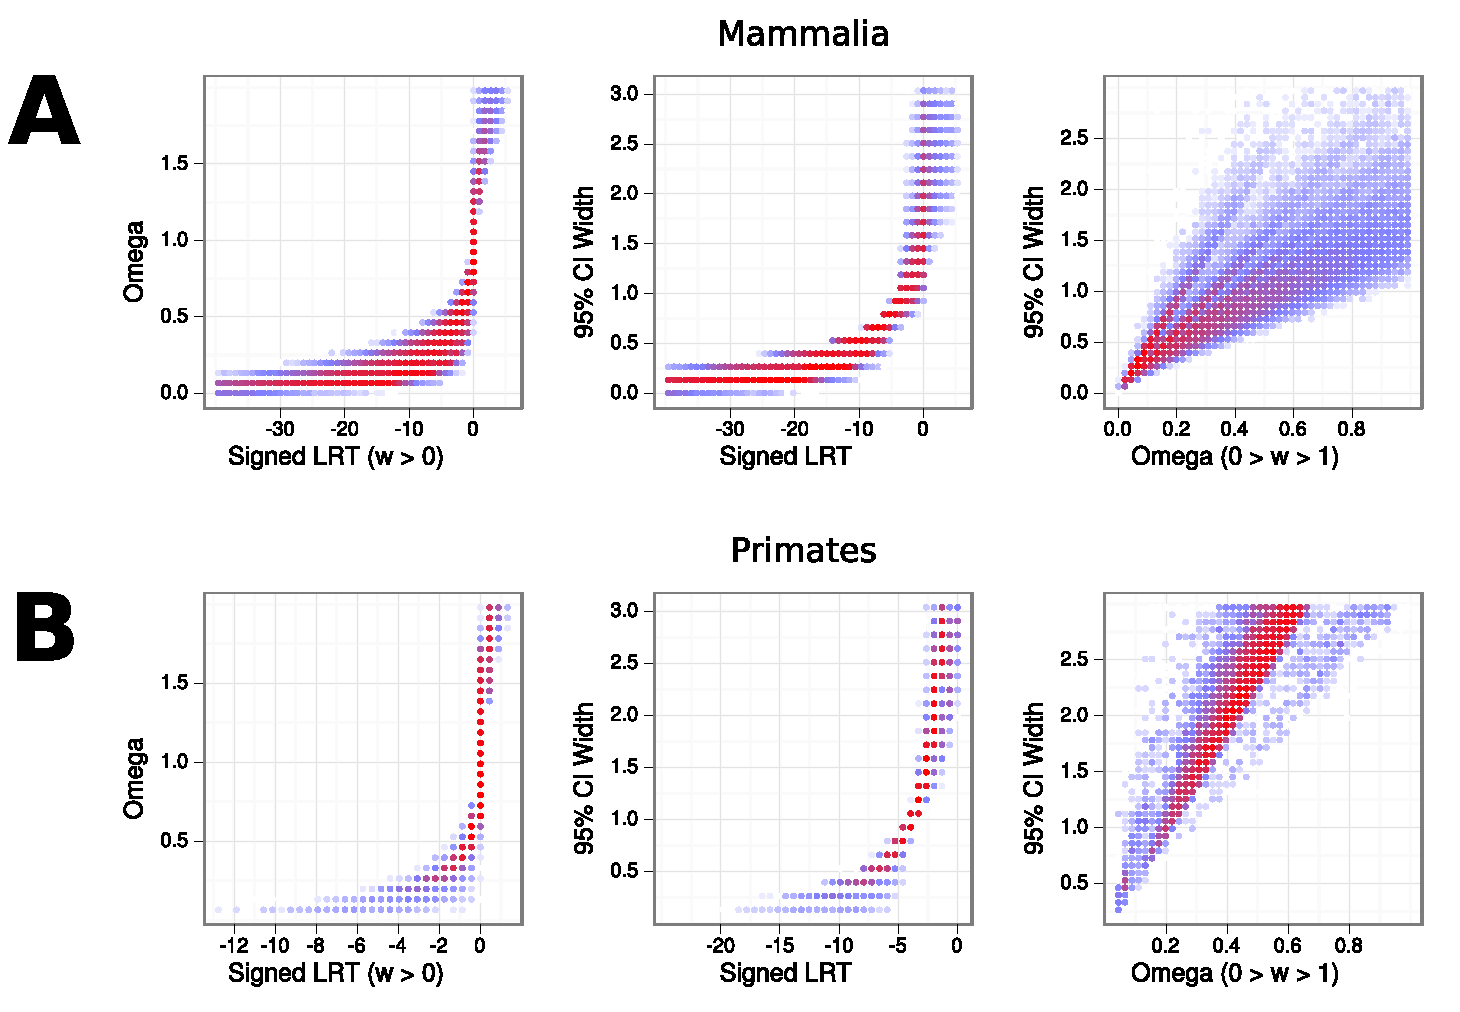
\includegraphics[scale=0.5]{Figs/sites_scatters.pdf}
\caption{The relationship between \slrt, \omgml, and \ci width in (A)
  Mammalia and (B) Primates datasets. Each point represents the binned
  density of sites; no points are drawn where no density exists, while
  blue and red points are drawn at areas of low and high density,
  respectively. The left panel shows sites where \omgml$<0$, the
  middle panel shows all sites, and the right panel shows sites where
  $0<$\xspace\omgml$<1$. Note the change in x-axis scales between plots
  in (A) and (B), reflecting the paucity of sites in Primates with
  strong evidence (\slrt$<$-12) for purifying selection.}
\label{fig_sites_scatters}
\end{figure}

To further explore this point, Figure \ref{fig_sites_scatters}A shows
the relationship between \slrt, \omgml and the \ci width for sites
from the Mammals group. The left panel, comparing the \slrt to \nz
\omgml estimates, shows that the two values are highly correlated,
with the greatest number of low \omgml estimates occurring at sites
with strongly negative \slrt{}s. Correspondingly, the middle panel
shows an even stronger relationship between the \slrt magnitude and
the \ci width, with the tightest confidence intervals at sites with
very strong evidence for purifying selection. The rightmost panel
compares the \omgml of each site with the width of its \ci, revealing
a more linear and diffuse positive relationship between \omgml and the
size of the \ci. The equivalent plots for Primates, shown in Figure
\ref{fig_sites_scatters}B, reveal similar patterns, but with generally
less-negative \slrt values, higher \omgml, and larger \ci. These
differences highlight the impact of branch length on the amount of
confidence with which \omg can be estimated on a per-site basis. The
low branch length of the Primates clade rarely yields \omgml estimates
with \ci intervals smaller than 1, while the bulk of sites from the
Mammalia dataset have relatively small \ci{}s. Thus, the distribution
of \omgml estimates from datasets with low branch lengths (e.g., the
histogram densities seen in Figure \ref{fig_global_distributions})
should be interpreted with caution, as any comparison between \omgml
from different sites or datasets may be more sensitive to the amount
of statistical confidence placed on each estimate than to any
meaningful biological difference between the two sets of data.


\bbtable
\scriptsize{ \centering
\begin{tabular}{lllrrrrrrrrrrrrr}
\toprule
 &  & &  \multicolumn{3}{c}{Site Pattern, \%} & Med. & 
  \multicolumn{3}{c}{Nongap BL} & \multicolumn{2}{c}{\omgml} &
\multicolumn{4}{c}{\omgml Below / Above, \%} \\
\cmidrule(r){4-6} \cmidrule(r){8-10} \cmidrule(r){11-12} \cmidrule(r){13-16}
Name & Filter & Sites & Const. & Syn. & Nsyn. & Codons & Med. & Mean & SD & Mean & SD &
$< 0.5$ & $< 1$ & $> 1$ & $> 1.5$ \\
  \midrule
\input{Tables/pset_summaries_stringent_1.txt}
\bottomrule
\end{tabular}
\caption{\scriptsize Summary statistics of \sw estimates for all
  species groups with the conservative filter applied. Columns under
  the ``\omgml Below / Above'' heading measure the percentage of sites
  with \omgml below or above the indicated value. Med.---median,
  Const.---constant, Syn.---\syn, Nsyn.---\nsyn, BL---branch length.
\label{table_pset_summaries_1}
}

\hspace{.2in}

\centering
\begin{tabular}{llrrrrrrrrrrrrrrrrrrrrr}
\toprule
 & & \multicolumn{8}{c}{Positively Selected Sites (\%)} &
\multicolumn{3}{c}{\chisqlt{0.1}, \%} &
\multicolumn{3}{c}{\chisqlt{0.05}, \%} \\
\cmidrule(r){3-10} \cmidrule(r){7-10} \cmidrule(r){11-13} \cmidrule(r){14-16}
Name & Filter & 
  \multicolumn{2}{c}{\chisqlt{0.1}} & \multicolumn{2}{c}{\chisqlt{0.05}} &
  \multicolumn{2}{c}{\chisqlt{0.01}}& \multicolumn{2}{c}{\bhfdr{0.05}} &
  Neg. & Neut. & Pos. & Neg. & Neut. & Pos. \\
%\cmidrule(r){2-3} \cmidrule(r){4-5} \cmidrule(r){6-7} \cmidrule(r){8-9}
\midrule
\input{Tables/pset_summaries_stringent_2.txt}
\bottomrule
\end{tabular}
\caption{\scriptsize Proportions of sites subject to positive, purifying and
  neutral selection at various \slrt thresholds. The
  Benjamini-Hochberg method \citep{Benjamini1995} was used to identify the
  \slrt threshold at which FDR$<$0.05. For columns under the headings
  ``\chisqlt{0.1}, \%'' and ``\chisqlt{0.05}, \%'', Pos. and Neg. are
  the percentage of sites with significant evidence for positive and
  negative selection, respectively, and Neut. is the percentage of
  ``neutral'' sites not showing significant evidence for non-neutral
  selection.}
\label{table_pset_summaries_2}
}
\eetable

Instead, the confidence intervals and \ac{lrt} statistics calculated
by \ac{slr} for each site could be used to identify sites evolving
under purifying or positive selection with confidence. Sites with
\ciup, the upper bound of the \ci interval, below \omg$=1$ could be
interpreted as having evidence of purifying selection with an expected
5\% \fpr; likewise, sites with \cidown above \omg$=1$ contained
evidence of positive selection with an expected 5\% \fpr. In both
cases, \ac{slr} was controlling for an expected 5\% \fpr under the
null model of neutral evolution. As expected, there was a direct
relationship between \ciup and the \chisq approximation to the \slrt
distribution, whereby the set of sites with \ciup$<1$ was exactly
equivalent to the set of sites with \slrt below the negative \chisq
95\% critical value. Similarly, the sites with \cidown$>1$ were those
with \slrt above the \chisq 95\% critical value. Because of this
equality, I will refer to \slrt values at various \chisq threshold
values instead of the 95\% \ci intervals when discussing sites with
significant evidence for purifying or positive selection.

Tables \ref{table_pset_summaries_1} and \ref{table_pset_summaries_2}
provide summaries of the sitewise estimates obtained for each of the
10 mammalian species groups, showing the same values provided earlier
in Tables \ref{table_filter_summaries_1} and
\ref{table_filter_summaries_2} for the different filters.

Table \ref{table_pset_summaries_2} presents the proportions of
\acp{psc} identified at a variety of \slrt thresholds, demonstrating
that anywhere between 0.01\% to 0.73\% of sites could be confidently
identified as under positive selection in mammals at nominal \ac{fpr}
thresholds between 1\% and 10\%. Interestingly, however, different
species groups yielded strikingly different estimates of the
proportion of \acp{psc}. At a 5\% FPR threshold, the Primates, HQ
Mammals, Laurasiatheria, Eutheria, and Mammals groups produced broadly
comparable proportions of positively-selected sites, ranging from
0.33\% to 0.42\%. The proportions of \acp{psc} in these groups were
higher using a 10\% FPR threshold (ranging from 0.46\% to 0.73\%) and
lower using a 1\% FPR threshold (ranging from 0.07\% to 0.19\%). When
the FDR was controlled using the Benjamini-Hochberg method, however,
far fewer \acp{psc} were identified. Only the Eutheria and Mammalia
groups yielded a substantial number of positively-selected sites at
this level of control; the Primates and Laurasiatheria data yielded
non-zero numbers of \acp{psc} as well, but these species groups were
likely limited in their power to yield positively-selected sites after
FDR control due to their lower total branch lengths.

The Atlantogenata, HMRD, Sparse Glires, Glires and Sparse Mammalia
groups all produced very low proportions of positively-selected sites
identified across all \fpr thresholds. At FDR$<$0.05, all four groups
yielded zero significant \psc{}s, and at a 1\% \ac{fpr} they all
contained lower than 0.01\% \acp{psc}. These \ac{psc}-depleted species
groups were widely distributed in the amount of total branch length
they covered (ranging in median \ngap branch length from 0.94 for
Atlantogenata to 2.55 for Sparse Mammals), suggesting that the lower
number of \acp{psc} was not strongly influenced by branch length; a
similar point could be made of the species groups with higher
proportions of \acp{psc}, which comprised the groups with the lowest
(Primates) and highest (Mammals) total branch length.

In Mammalia, the breakdown of sites into positive, negative and
neutral categories at 10\% and 5\% significance thresholds produced a
pattern similar to that seen in the \omgml distributions from Figure
\ref{fig_global_distributions}, with a large amount of purifying
constraint (83.87\% of sites at 5\% FPR), a small proportion of
neutrally-evolving sites (15.57\%), and a diminishing number of
positively-selected sites (0.55\%). As expected given the use of a
fixed \slrt threshold to identify purifying sites, the fraction of
sites confidently identified as under purifying selection showed a
strong dependency on the branch length of the species set, with a much
higher power in Mammalia than in Primates to confidently detect
purifying selection (83.87\% vs. 15.97\%).

Overall, the conservatively-filtered \sw data showed that, when using
\omgml estimates, between 1\% to 5\% of protein-coding sites are
evolving under positive selection. This number varied strongly between
different species groups, however. Comparing between the four
phylogenetically independent mammalian superorders (Primates, Glires,
Laurasiatheria, and Atlantogenata), I found that Primates showed by
far the most \acp{psc} and sites with \omgml$>1$. Laurasiatheria
showed similar proportions of sites with \omgml$>1$, but Atlantogenata
showed fewer \acp{psc} than Laurasiatheria; this difference may
reflect their different branch lengths, as the Laurasiatheria group
covers twice as much branch length as Atlantogenata and thus would be
expected to have more power to confidently detect positive
selection. Finally, the Glires group showed strikingly lower levels of
positive selection compared to the other mammalian
superorders. Despite the relatively high branch length contained
within Glires (median total length of 1.77 versus 2.03 for
Laurasiatheria), only 0.10\% of sites were identified as \acp{psc} in
Glires at a 5\% \ac{fpr}, compared to 0.33\% in Laurasiatheria and
0.41\% in Primates.

These results may be evaluated in terms of the impact of effective
population size on the efficacy of natural selection in mammals
\citep{Popadin2007,Nikolaev2007,Ellegren2009}. Rodents are known to
have an effective population size well above that of primates
\citep{Kosiol2008}, and given the strong correlation between body
size, generation time and effective population size
\citep{Nikolaev2007}, one can infer that species within the
Laurasiatheria group, with generally longer generation times and
larger body sizes than rodents \citep{Hou2009}, have effective
population sizes more similar to those seen in primates. The
Afrotheria group, containing species ranging from small moles to
elephants and manatees, is more diverse, making it difficult to
estimate an expected historical effective population
size. Nevertheless, Ohta's nearly neutral theory \citep{Ohta1992}
predicts that species with lower effective population sizes will
evolve with less efficient natural selection. A comparison of the
Primates and Glires data clearly revealed this effect: the proportion
of sites with \omgml~$<0.5$ was 87.27\% for Primates and 90.54\% for
Glires. Thus, the difference in the proportion of sites likely to be
under purifying selection was well-explained by the difference in
effective population size between primates and rodents. If the
existence of \acp{psc} in the \sw data is interpreted as true evidence
for positive selection, then the nearly neutral theory predicts that
Glires should show \emph{more} \acp{psc} than Primates, as the
efficacy of positive selection would be greater in the species with a
larger effective population size. The opposite effect is seen,
however, with Primates showing much greater levels of apparent
positive selection as measured by both the proportion of sites with
\omgml$>1$ and by \acp{psc} identified at various \ac{fpr} thresholds.

This suggestes an alternative interpretation: that perhaps the
different levels of positive selection could be due mainly to the
relaxation of selective constraint in Primates and other species with
low effective population sizes. A difference in effective population
sizes should have its main effect on slightly deleterious mutations,
with a greater proportion of slightly deleterious mutations (e.g.,
mutations with fitness effects corresponding to \dnds values slightly
below 1) becoming effectively neutral in a species with a low
effective population size. In comparing the Primates and Glires
groups, the expected result is that a subset of mutations which were
under purifying selection in Glires would be effectively neutral in
Primates, bringing the expected \omg from $<1$ to 1. If this class of
sites were large enough, it might significantly interfere with the
resulting \ac{fpr} for detecting \acp{psc}, as sites with \omg$=1$ are
the most prone to produce false positives.

Thus, the relaxed constraint argument tempers the interesting
observation of strong differences in the numbers of \acp{psc} between
different species groups. A lower historical effective population size
for the Primates and Laurasiatheria species groups may explain some of
the increase in the number of \acp{psc} detected, even in the absence
of true variation in the prevalence of positive selection between the
species groups investigated here. Still, the argument may be made that
statistical methods for controlling error rates, such as the
Benjamini-Hochberg method for FDR control used to identify \acp{psc}
at an expected FDR$<0.05$ in Table \ref{table_pset_summaries_2}
\citep{Benjamini1995}, should account for the potential confounding
effects of relaxed constraint noted above. For this reason, the
observation that Primates and Laurasiatheria both yielded non-zero
numbers of \acp{psc} at FDR$<0.05$ may be taken as some indication of
a true difference in the levels of positive selection between the
species groups investigated here.

\section{Conclusions}

This chapter described the filtering, alignment, and analysis of a
comprehensive set of mammalian orthologs across 38 species.

In order to ensure that false signals of positive selection were
avoided as much as possible, several levels of filtering were applied
before and after the estimation of \sw selective pressures using
\ac{slr}: low-quality genomic sequence was masked out, short or
divergent apparent paralogous copies were removed, and alignment
columns showing evidence of clustered \nsyn substitutions or low
amounts of evolutionary information were excluded from the analysis. A
comparison of the levels of purifying and positive selection contained
within sites filtered at various thresholds showed the importance of
thorough filtering prior to genome-wide analysis, highlighting
especially the ability of stretches of mis-annotated or mis-assembled
sequence to introduce strong (and incorrect) signals of localized
positive selection into evolutionary analyses. I showed that a novel
approach, based on the identification of lineage-specific clusters of
excessive \nsyn substitutions within short alignment windows, could
effectively target these erroneous regions for removal.

I applied the conservative filter to sitewise estimates obtained from
several groups of mammalian species. This allowed the impact of the
total branch length of a species group on the estimation of \sw
selective pressures to be clearly seen, with the Mammals group
containing many more non-constant alignment sites and more realistic
\omgml estimates than groups with little branch length, such as
Primates. Relating my results back to the \ac{mgp}, which used the
HMRD and HQ Mammals groups as reference points by which to estimate
the increase in power to detect genome-wide constraint resulting from
the additional mammals sequenced at low coverage, I found that the
addition of \lcv genomes increased the ability to detect purifying
constraint in protein-coding regions by 43.85\% and 136\% compared to
the HQ Mammals and HMRD species groups, respectively, at a 5\%
\ac{fpr}. Although I found the levels of positive selection between
species groups to be highly dependent on the species sampling (and
thus, a comparison of ``power'' to be less meaningful), the Mammals
species group identified 21.5\% and 550\% more \acp{psc} than the HQ
Mammals and HMRD species groups, respectively, at a 5\%
\ac{fpr}. Thus, the additional branch length resulting from the
sequencing of \lcv genomes greatly improved the power to detect
purifying and positive selection in mammalian proteins.

Finally, I analyzed the levels of purifying and positive selection
within four phylogenetically independent mammalian species groups,
identifying strong differences between different groups, likely
resulting from differences in effective population size. Although the
impact of effective population size is well known and has been
previously studied in mammalian superorders, the work described in
this chapter represented a careful and quantitative analysis of levels
of purifying and positive selection in these species groups. The
observation that the Glires group showed less positive selection than
all other groups suggested a connection between high numbers of
\acp{psc} and relaxed constraint, although Primates and Laurasiatheria
both showed evidence for strong \acp{psc} even at a very stringent FDR
threshold.

Although more work needs to be done to evaluate what might be causing
these differences between species and to correctly control for the
possible effects of relaxed constraint, I have shown that the analysis
of \sw estimates is an intuitive and informative approach to
evaluating signals of purifying and positive selection in mammalian
genomes.

\tocite{Eory et al. 2010}{Showed, through constraint analysis of
  various sequence types, that there is higher selective constraint in
  4-fold sites in priamtes compared to murids. Quote: ``It is well
  established that in several organisms, mutations at 4-fold sites are
  selected against (Chamary et al. 2006; Rocha 2006; Drummond and
  Wilke 2008) and as a consequence the dN/ds ratio, which has been
  frequently used to detect the strength and direction of selection
  (e.g., Dorus et al. 2004; Wang et al. 2006), may be
  underestimated. Our result of higher 4-fold constraint in hominids
  suggests that this bias more strongly affects hominid estimates and
  it may well exceed 20\%.''}

\tocite{Ohta 1993, 1995; Eory et al. 2010}{The Keightley et al. 2011
  paper (ABC to estimate mutation rate parameters) cited Ohta 1993,
  1995 and Eory et al. 2010 for the effective population size and
  efficacy of selection in primates vs. murids}

\tocite{Wolf et al. 2009}{Wolf et al. GBE 2009, used pairwise dN dS
  counts to try to show that trends in dN/dS ratios are a result of
  branch length, at least when calculated in a pairwise
  fashion. Slightly unconvincing stuff... could be cited as somehow
  relating to the discussion regarding eff. pop. size, branch length,
  and selection}

\tocite{Berglund et al. 2009}{Berglund et al. 2009 looked at hotspots
  of biased substitutions in humans. Showed that exons with
  accelerated rates in humans have a tendency towards clusters of
  AT-to-GC (weak-to-strong) substitutions. Did some simulations
  showing that this effect is strongest in GC-poor regions, though the
  impact on overall dN/dS is probably minimal (e.g., genes with
  overall high dN/dS didn't show BGC, only the most accelerated exons
  did) and the effect on dN/dS is highest in high-GC regions. The
  most-accelerated exons tend to reside in high-male (but not female)
  recombination, and <50kb from hotspots. Upshot: these biased
  clusters seem to show up in isolated regions (exons), rather than
  spread throughout entire genes. Probably not a huge impact on
  overall apparent constraint.}

\tocite{Duret and Arndt PLoS Gen 2008}{Duret and Arndt 2008 use
  nonreversible nucleotide models to estimate NEUTRAL rates correlated
  with recombination, GC, and GC*. Lots of stuff here, but the
  important bits: overall mutation rate increases with increasing GC
  content (due to overall higher rates of S-W substitution);
  recombination should have a strong impact on W-S substitution, but
  weak impact on S-W substitutions; CpG deamination varies by factor
  of two, very low in GC-poor regions and very high in GC-rich ones.}

\tocite{Galtier et al. TrIG 2009}{Galtier et al. TRIG 2009 is similar
  to Berglund et al. in many ways -- find accelerated exons in a
  primate branch, and identify significantly higher male recombination
  rates there. The number of accelerated exons is small -- ~100 in
  each of four branches -- and not all of these accelerated exons
  showed strongly elevated dN/dS ratios. Only 19 exons at the 1\%
  level. However, they do some nice modeling (mostly in the
  supp. material) which shows that the effect of BCG on dN/dS ratio at
  different GC contents -- it has more effect in GC-rich genes.}

\tocite{Capra and Pollard 2011}{Capra and Pollard quantified BDS
  (biased divergent substitutions) across metazoans, additionally
  using recombination rate data. Dog has the strongest, mouse has the
  weakest BDS scores. (This could be due to lower rec. rate in mouse,
  e.g. Coop and Przeworski 2006)}

\tocite{Nordborg et al. 1996}{Nordborg et al. 1996 (Genet. Res.)
  modeled the effect of background selection on variation in neutral
  linked loci. They showed that weakly selected mutations, rather than
  strongly selected ones, are more likely to produce regional
  patterning of variation in response to local recombination
  rate. Should have a large effect in Drosophila but small effect in
  mammals, though in mammals ``local reductions in regions of reduced
  recombination might be detectable.''}

\tocite{Chun and Fay 2011}{Chun and Fay 2011 (PLoS Gen) looked at
  neutral and deleterious SNP density according to local recombination
  rate, showing that in 'hitchhiking' regions there are fewer neutral,
  but as many deleterious, polymorphisms. That stuff is boring, but
  they also show that the deleterious SNP density stays constant
  throughout the range of recombination rates, while the neutral and
  synonymous SNP density decreases. Thus, slightly deleterious
  mutations are less effectively purged in regions of low
  recombination.}

\tocite{Bullaughey et al. 2008}{Bullaughey et al. (2008, Gen. Res.)
  looked at gene-wide dN/dS ratios in primates and recombination
  rates. They found no significant correlation between broad- or
  fine-scale recomb. rates and rates of protein evolution, **once GC
  content is taken into account**.}

\tocite{SPencer et al. 2006}{Spencer et al. (2006 PLoS Gen) Quote: ``In short,
  while there is a strong relationship between recombination and GC
  content, most of the relationship is explained by scales broader
  than recombination hotspots (16 to 256 kb; unpublished data) and may
  well result from interactions of both factors with additional
  processes such as chromatin organisation or replication
  timing. Similar arguments apply to the question of whether a GC bias
  in recombination-associated mutation can explain the relationship
  between GC content and recombination.''}

\draft{...}

